\chapter{Accelerating Convolutional Neural Networks for FPGA using Depthwise Separable Convolution and Pruning} \label{chap:pratique}
%
%
In the previous chapter, we introduced pruning, which reduces both size and computational complexity of \acrshort{cnn}s. We also showed that there exist various pruning schemes. Each of them can be categorized from coarse-grained to fine-grained. Coarse-grained pruning schemes have the advantage that they can be easily implemented on \acrshort{gpu} and \acrshort{cpu} in exchange for a drop of accuracy. On the other hand, fine-grained pruning schemes can limit this reduction of accuracy but create irregular access pattern that makes them difficult to implement on such platforms. 

To have an efficient \acrshort{fpga}-based accelerator, we should focus on implementing the most fine-grained pruning scheme possible to apply a high sparsity while limiting the loss of accuracy. This shows the advantage of using \acrshort{fpga} accelerator because, as said previously, this type of pruning scheme is not easily implementable on \acrshort{cpu} and \acrshort{gpu}

In this chapter, we define an \acrshort{fpga}-based accelerator architecture that integrates both pruning and \acrshort{dsc} (see Section \ref{subs:dsc} )to further reduce the number of weights and operations. To show its applicability, this architecture implements a state-of-the-art network that includes \acrshort{dsc} and targets embedded platforms: MobileNetV2 (see Sections \ref{subs:mbv2} and \ref{subsec:mdopti}). Since the pruning can cause a degradation of the performance, we have to determine the design objectives of the architecture and its associated pruning scheme, which are the following:
%
\begin{enumerate}
    \item The pruning scheme is as fine-grained as possible.
    \item The pruning scheme reduces the computational complexity.
    \item The pruning scheme allows a reduction of the memory required to store the weights.
    \item The proposed architecture provides a logically correct output.
    \item An increase in the sparsity improves the performance of the architecture.
\end{enumerate}
%
Section \ref{sec:design} aims at developing the pruning scheme and the algorithm to handle it. We also define in this section the reduction factors of weight and operations when using the proposed pruning scheme. We also define a weight compressed format to reduce weight memory use. We then perform a loop analysis on the proposed algorithm to determine the optimal hardware design variables and the structure of the architecture.

Section \ref{sec:implementation} describes the implementation of the accelerator \acrshort{fpga}-based architecture and details its dataflow. We start by explaining the overall architecture and then we go into each component.

Section \ref{sec:measure} shows the results obtained and discusses if the proposed design objectives are met.
%
\section{Design of a FPGA-based accelerator integrating structured sparse DSC} \label{sec:design}
%
As previously said,  the aim of this section is to develop a pruning scheme for the \acrshort{dsc} that fulfills the design objectives and an algorithm able to support it. First, we detail the pruning scheme used and the weights and operations reduction factors obtained by applying the pruning. Second, we analyse the sparse kernels to find a compressed format that reduces the memory use and overhead of determing the address of the non-pruned weights. Third, we describe the algorithm proposed to perform the sparse \acrshort{dsc} using the proposed pruning scheme. Finally, we analyse the convolution loops to determine the optimal design of the \acrshort{pe} that perfoms the convolution.
%
\subsection{Pruning scheme} \label{subsec:pscheme}
%
\acrshort{dsc} is composed of two types of convolution: depthwise and pointwise convolutions (see Section \ref{subsec:layer}). We decided to apply pruning on the pointwise filters for the following reasons:
%
\begin{itemize}
    \item In MobileNet and MobileNetV2, most of the operations are done in the pointwise convolutions \cite{zhang_channel_2019, tu_pruning_2019}. So it is the operation where the reduction of weights and computational complexity would be the most relevant (each operation requires one weight).
    \item As each kernel of pointwise filter is a vector of size $1 \times 1  \times N_{if}$, we therefore have to prune in the channel-axis. This scheme was proven to be successful by \textcite{kang_accelerator-aware_2020}.
    \item The pruning scheme can be applied to each $1 \times 1$ convolution in the network.
\end{itemize}
%
As mentionned above, we decided to develop a pruning scheme inspired by the methodology of \textcite{kang_accelerator-aware_2020}, which prunes weights in the channel-axis.

Ideally, without pruning, each \acrshort{pe} performing a pointwise convolution fetches $N_{if}$ weights and input pixels belonging to spatial coordinates $(x, y)$ (pointwise convolution only convolves pixels in the channel-axis). Then each weight is multiplied with its corresponding pixel and the products are summed to obtain one output pixel of one channel. If we apply an unstructured pruning on the pointwise filter, we can use the same algorithm as above but only each non-pruned weight is multiplied with its corresponding pixel (multiplication implying zero-value weights can be safely discarded).

However, as the resources of the \acrshort{fpga} are limited, the \acrshort{pe} can only fetch $N_{par} \leq N_{if}$ weights and pixels at each time (which corresponds to a \textbf{fetching group}; each input \acrshort{fm} and kernel are composed of $N_{gr}$ fetching groups). Therefore, we would do the convolution between each fetching group and accumulate the different partial sums belonging to a same output pixel until an output pixel is produced. If an unstructured pruning is applied, this can cause several issues, as pointed out by \cite{kang_accelerator-aware_2020}.

First, it can cause misalignement between the weight and pixel fetching groups. Indeed if we prune the first $N_{par}$ weights in the kernel, the first pixel fetching group is useless. Second, there can be a load-imbalance problem (see Section \ref{subsec:impl_prun}) that can occur between two \acrshort{pe}s if the number of pruned weights between two kernels is different. 

To solve these problems, the solution proposed by \textcite{kang_accelerator-aware_2020} is to align pixel and weight fetching groups. Each pixel fetching group has a corresponding weight fetching group containing at least one non-pruned weight. \textcite{kang_accelerator-aware_2020} also constrains the number of non-pruned weights in each fetching group to be the same number, called $N_{np}$. Therefore, it solves also the load-imbalance problem. As a result, the proposed sparse \acrshort{dsc} can be illustrated in Figure \ref{fig:prunedwg}.
%
\begin{figure}[H]
    \centering
    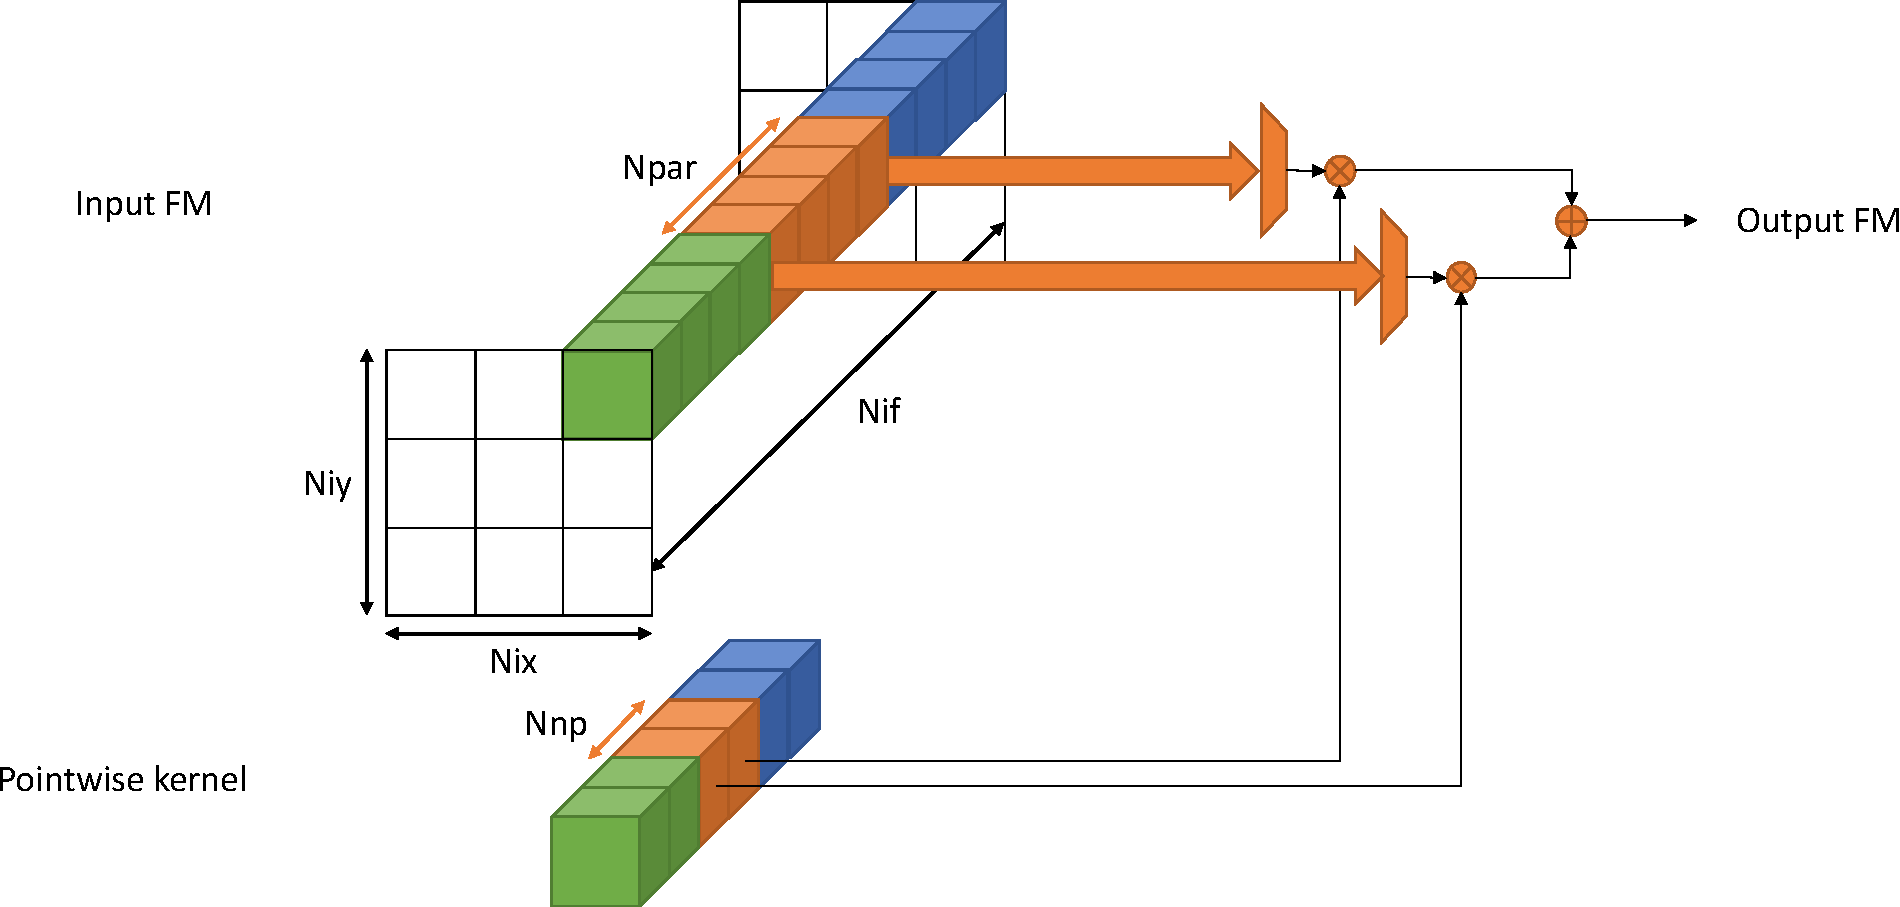
\includegraphics[width=\textwidth]{pruningscheme.pdf}
    \caption{Process of a pointwise convolution with a sparse pointwise kernel, inspired by \cite{kang_accelerator-aware_2020}}
    \label{fig:prunedwg}
\end{figure}
%
To summarize, each pointwise kernel is composed of $N_{gr}$ fetching groups of $N_{np}$ weights. Each group corresponds to a pixel fetching group of size $N_{par}$. We define the ratio between the number of non-pruned weights and the size of the fetching group without pruning as the \textbf{pruning ratio $\alpha$}, the number of weights remaining after pruning. The ratio of pruned weights is therefore equal to $1 - \alpha$. The pruning parameters are defined in Table \ref{tab:pr_param}. Moreover, the proposed pruning scheme can also be applied to each $1 \times 1$ kernels.
%
\begin{table}[H]
    \center
    \begin{tabular}{|c|c|c|}
        \hline
        $N_{par}$ & The input pixel fetching group size. & $N_{par} \leq N_{if}$ \\
        \hline
        $N_{np}$  & The pointwise weight fetching group size. & $N_{np} \leq N_{par}$ \\
        \hline
        $N_{gr}$  & The number of fetching groups & $N_{gr} = \left\lceil \frac{N_{if}}{N_{par}} \right\rceil $ \\
        \hline
        $\alpha$  & The pruning ratio & $\alpha = \frac{N_{np}}{N_{par}}  $ \\
        \hline
    \end{tabular}
    \caption{Pruning parameters}
    \label{tab:pr_param}
\end{table}
%
We should add that this pruning scheme is not the same as \textit{channel pruning} since we do not constrain the same weights to be pruned in each group. Therefore, I did not consider the pruning of the depthwise kernel associated to the pruning of a weight in each kernel, as discussed in Section \ref{subs:pruning}. We have then proposed a pruning-scheme that is not coarse-grained (channel pruning), satisfying first design objective: \textbf{\textquote{The pruning scheme is as fine-grained as possible}}.
%
\subsubsection{Reduction factors}
%
We can now evaluate the reduction factors of the sparse \acrshort{dsc} compared with the \acrshort{dsc} without pruning and the standard convolution.

We consider that the size of the input feature map of the pointwise convolution is $N_{ix}  \times N_{iy} \times N_{if}$, the size of the depthwise filter is $N_{kx} \times N_{ky} \times N_{if}$, the size of the non-pruned pointwise convolution $N_{if} \times N_{of}$, the fetching group size is $N_{par}$, the number of pruned weights is $N_{np}$, and the size of the output \acrshort{fm} is $N_{ox}  \times N_{oy} \times N_{of}$. The amount of weights $W_{DSC}$ and operations $O_{DSC}$ of the \acrshort{dsc} can be determined using Equation \eqref{eq:dsc_wg} and \eqref{eq:dsc_op} \cite{bai_cnn_2018, liu_fpga-based_2019}.
%
\begin{equation}
    W_{DSC} = N_{kx} \times N_{ky} \times N_{if} + N_{if} + \times N_{of}
    \label{eq:dsc_wg}
\end{equation}
%
\begin{equation}
    O_{DSC} = N_{ix} \times N_{iy} \times N_{kx} \times N_{ky} \times N_{if} + N_{ix} \times N_{iy} \times N_{if} \times N_{of}
    \label{eq:dsc_op}
\end{equation}

In a same manner, the amount of weights $W_{PR\_DSC}$ and operations $O_{PR\_DSC}$ of the sparse \acrshort{dsc} can be determined using Equation \eqref{eq:pr_dsc_wg} and \eqref{eq:pr_dsc_op}.
%
\begin{equation}
    W_{PR\_DSC} = N_{kx} \times N_{ky} \times N_{if} + \times N_{if} + N_{np} \times N_{gr} \times N_{of}
    \label{eq:pr_dsc_wg}
\end{equation}
%
\begin{equation}
    O_{PR\_DSC} = N_{ix} \times N_{iy} \times N_{kx} \times N_{ky} \times N_{if} + N_{ix} \times N_{iy} \times N_{gr} \times N_{np} \times N_{of}
    \label{eq:pr_dsc_op}
\end{equation}

Thus, the weights $F_{Wg}$ and operations $F_{Op}$ reduction factors can be expressed according to Equation \eqref{eq:factor_comp_wg} and \eqref{eq:factor_comp_op}. The demonstration allowing to find these relations can be found in Appendix \ref{appendix:factor}.
%
\begin{equation}
    F_{Wg} = \frac{W_{DSC}}{W_{PR\_DSC}} = \frac{1 + \frac{N_{kx} \times N_{ky}} {N_{of}}} {\alpha + \frac{N_{kx} \times N_{ky}} {N_{of}}}
    \label{eq:factor_comp_wg}
\end{equation}
\begin{equation}
    F_{Op} = \frac{O_{DSC}}{O_{PR\_DSC}} = \frac{1 + \frac{N_{kx} \times N_{ky}} {N_{of}}} {\alpha + \frac{N_{kx} \times N_{ky}} {N_{of}}}
    \label{eq:factor_comp_op}
\end{equation}

As the reduction factors depend on the pruning ratio $\alpha$ and the number of output channels $N_{of}$, we can illustrate the evolution of the reduction factors depending on this parameter and the different $N_{of}$ of MobileNetV2. This can be seen in Figure \ref{fig:redfacto}.
%
\begin{figure}[H]
    \centering
    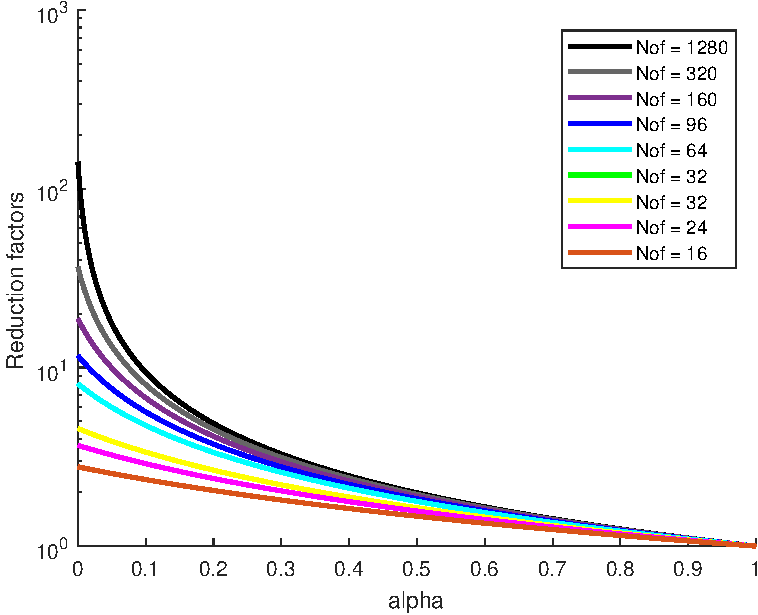
\includegraphics[width=0.75\textwidth]{RedFactor.pdf}
    \caption{Evolution of the reduction factors depending on the pruning ratio and the number of output channel}
    \label{fig:redfacto}
\end{figure}

For example, if we apply a pruning ratio of $25\%$ (meaning keeping $25\%$ of the weights in each fetching group), the reduction factors compared the \acrshort{dsc} without pruning are between two and four times. If we consider the reduction factor between \acrshort{dsc} and standard convolution is about 9 times \cite{zhang_channel_2019}, the reduction factors between sparse \acrshort{dsc} and standard convolution is between 18 and 36 times (if $\alpha = 25\%$). We therefore validated the second design objective, which is: \textbf{\textquote{The pruning scheme reduces the computational complexity}}.
%
\subsection{Compressed format} \label{subs:compress_f}
%
After applying the pruning scheme on the pointwise kernels, these kernels become sparse. This means that they contain zero-value weights, as illustrated in Figure \ref{fig:pruned_wg}. Therefore, in order to reduce the memory usage, we should only store each non-pruned weights in a compressed format that allows finding its address with no extra-overhead.
%
\begin{figure}[H]
    \centering
    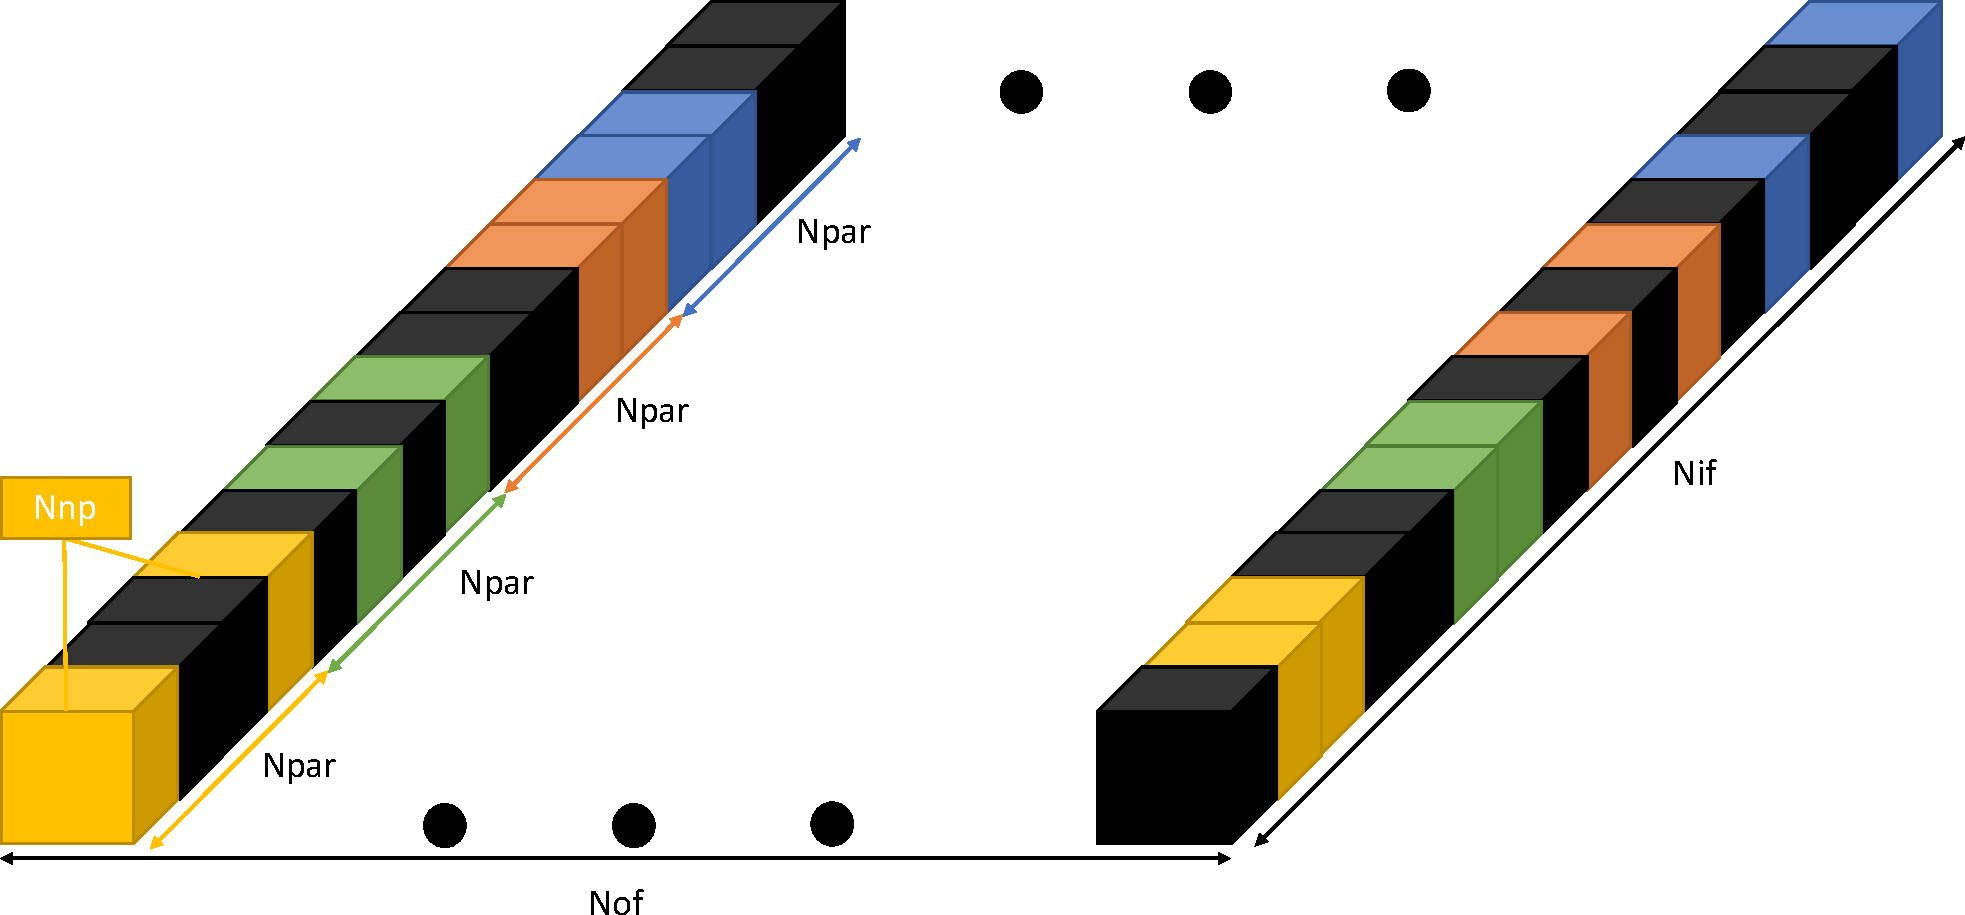
\includegraphics[width=0.75\textwidth]{pruned_wg.pdf}
    \caption{A pointwise kernel after pruning, where black cubes are pruned weights}
    \label{fig:pruned_wg}
\end{figure}

A conventional storage format for sparse matrix is the \acrfull{csr} \cite{buluc_parallel_2009}. According to \textcite{buluc_parallel_2009}, \textquote{\textit{The compressed sparse row (CSR) format stores the nonzeros (and ideally only the nonzeros) of each matrix row in consecutive memory locations,  and  it  stores  an  index  to  the  first  stored  element of each row}}. In other words, we represent a sparse matrix using three vectors:
%
\begin{itemize}
    \item \textbf{Vector val}: containing all the values of the non-pruned weights.
    \item \textbf{Vector col\_ind}: contains the column indices of the elements in \textbf{val}.
    \item \textbf{Vector row\_ptr}: contains the index of each row in \textbf{val}.
\end{itemize}
%
However, as for \cite{zhu_efficient_2020}, the \acrshort{csr} format can be compressed further thanks to the pruning scheme. Indeed, since the kernels to compress are vectors, we can reduce the storage usage by removing the \textbf{row\_ptr} vector (the kernel has only one row). 

Moreover, we can have a better compression if we reduce the number of bits allocated to represent the column index of a weigth. Indeed, without pruning, as each weight belongs in a fetching group of size $N_{par}$, it is sufficient to store the position of the weight in that group, instead of its asbolute position in the kernel. As a result, we can reduce the number of bits from $log_2(N_{if})$ (asbolute position) to $log_2(N_{par})$ (relative position), where $N_{par} \leq N_{if}$. Moreover, it also reduces the overhead to find the corresponding pixel in a fetching group, for each weight.

In brief, each sparse kernel is converted into 2 vectors of size $N_{np}$: vector \textbf{val}, which contains the value of the non-pruned weights, and vector \textbf{position}, which contains the position of the corresponding pixel in a fetching group. An example is illustrated in figure \ref{fig:compressed_format}.
%
\begin{figure}[H]
    \centering
    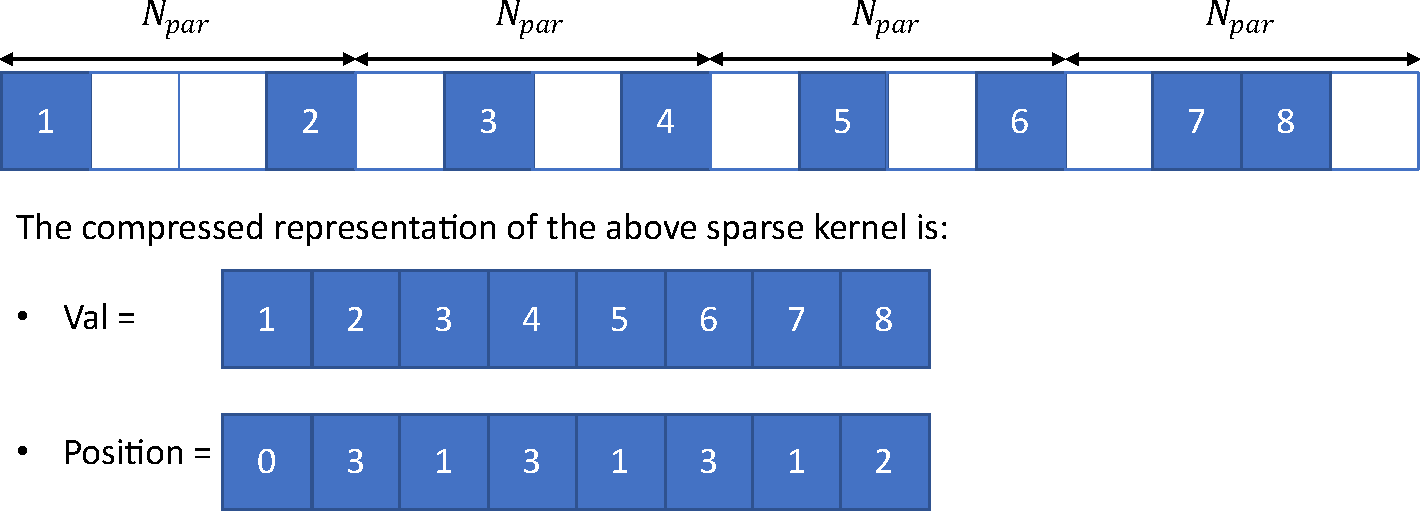
\includegraphics[width=0.75\textwidth]{compressed_format.pdf}
    \caption{Illustration of the compressed format on an example, where $N_{par} = 4$ and $N_{np} = 2$}
    \label{fig:compressed_format}
\end{figure}

Since this compressed format requires an extra position per weight (and hence more bits allocated per weight), we computed the maximal pruning ratio, or in a same way the minimal ratio of pruned weights, required to have a reduction of the memory usage. The relation between maximal pruning ratio and memory reduction can be found in Equation \eqref{eq:prun_mem} where $BW_{weight}$ is the bitwidth required to represent the value of a weight. The demonstration to find the maximal pruning ratio $\alpha$ to reduce the memory usage can be found in Appendix \ref{appendix:cf}.
%
\begin{equation}
    \alpha < \frac{BW_{weight}}{ BW_{weight} + log_2(N_{par})}
    \label{eq:prun_mem}
\end{equation}

The curve representing the minimal ratio of pruned weight, equals to $1 - \alpha$, depending on $N_{par}$ when $BW_{weight} = 16$ is illustrated in Figure \ref{fig:prun_mem}. We can conclude from the curve that we need to have a ratio of pruned weights to be greater or equal than $40\%$ in order to save memory. We can also conclude that we can prune less weights if we reduce the value of $N_{par}$. We therefore validated the third design objective, which is: \textbf{\textquote{The pruning scheme allows a reduction of the memory required to store the weights}}.
%
\begin{figure}[H]
    \centering
    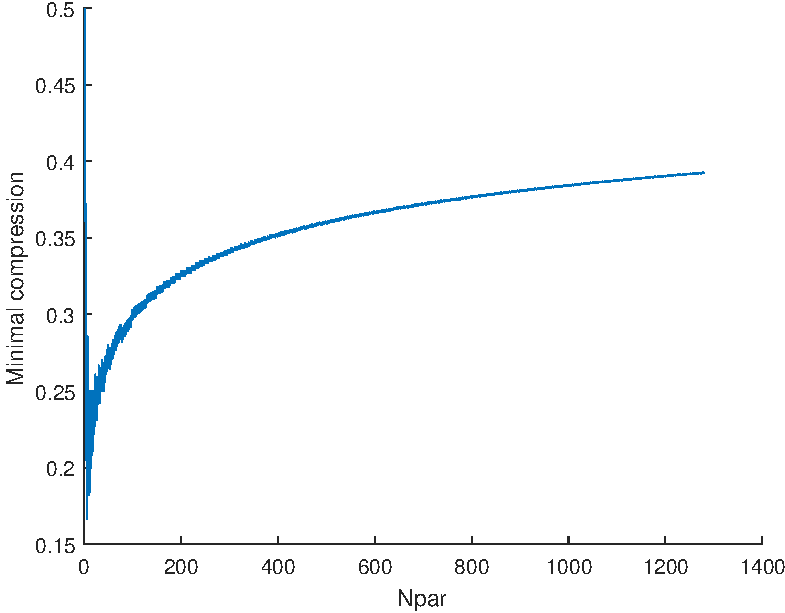
\includegraphics[width=0.75\textwidth]{MinCompr.pdf}
    \caption{Minimal ratio of pruned weights if $BW$ = 16}
    \label{fig:prun_mem}
\end{figure}
%
\subsection{Adding the pruning scheme to MobileNetV2} \label{subsec:mbnv2-pr}
%
As we have seen how the weights of a $1 \times 1$ kernel are pruned and explained the compressed format of the kernels, we present in this section how to integrate the proposed pruning scheme into MobileNetV2. In MobileNetV2, the \acrshort{dsc} layer is included into a larger building block, the \textit{inverted residual block} which performs the bottleneck convolution (see Section \ref{subs:mbv2}). In the bottleneck convolution, the \acrshort{dsc} follows a $1 \times 1$ convolution layer that expands the number of input channels by a factor t. As a result, we have to compute two sparse $1 \times 1$ convolutions. We note that the \acrshort{fm} produced by the $1 \times 1$ convolution is referenced as \textbf{intermediate \acrshort{fm}} in the rest of this thesis. The intermediate \acrshort{fm} is composed of $N_{gr_{int}} = t \times N_{gr}$ fetching groups, which are fed to the \acrshort{dsc}.

As explained in Section \ref{subsec:pscheme}, each $1 \times 1$ and pointwise convolutions have to fetch $N_{par}$ input pixels in the channel-axis, which corresponds to $N_{par}$ channels. Consequently, if the $1 \times 1$ convolution produces $N_{par}$ channels, the \acrshort{dsc} can fetch those intermediate products to produce partial results of the output \acrshort{fm}. Indeed, we can perform the depthwise convolution with each intermediate channel and then perform the pointwise convolution with the corresponding weight in each pointwise kernel, as illustrated in Figure \ref{fig:algo}. The output \acrshort{fm} is computed when the \acrshort{dsc} has performed these steps for each intermediate group.
%
\begin{figure}[H]
    \centering
    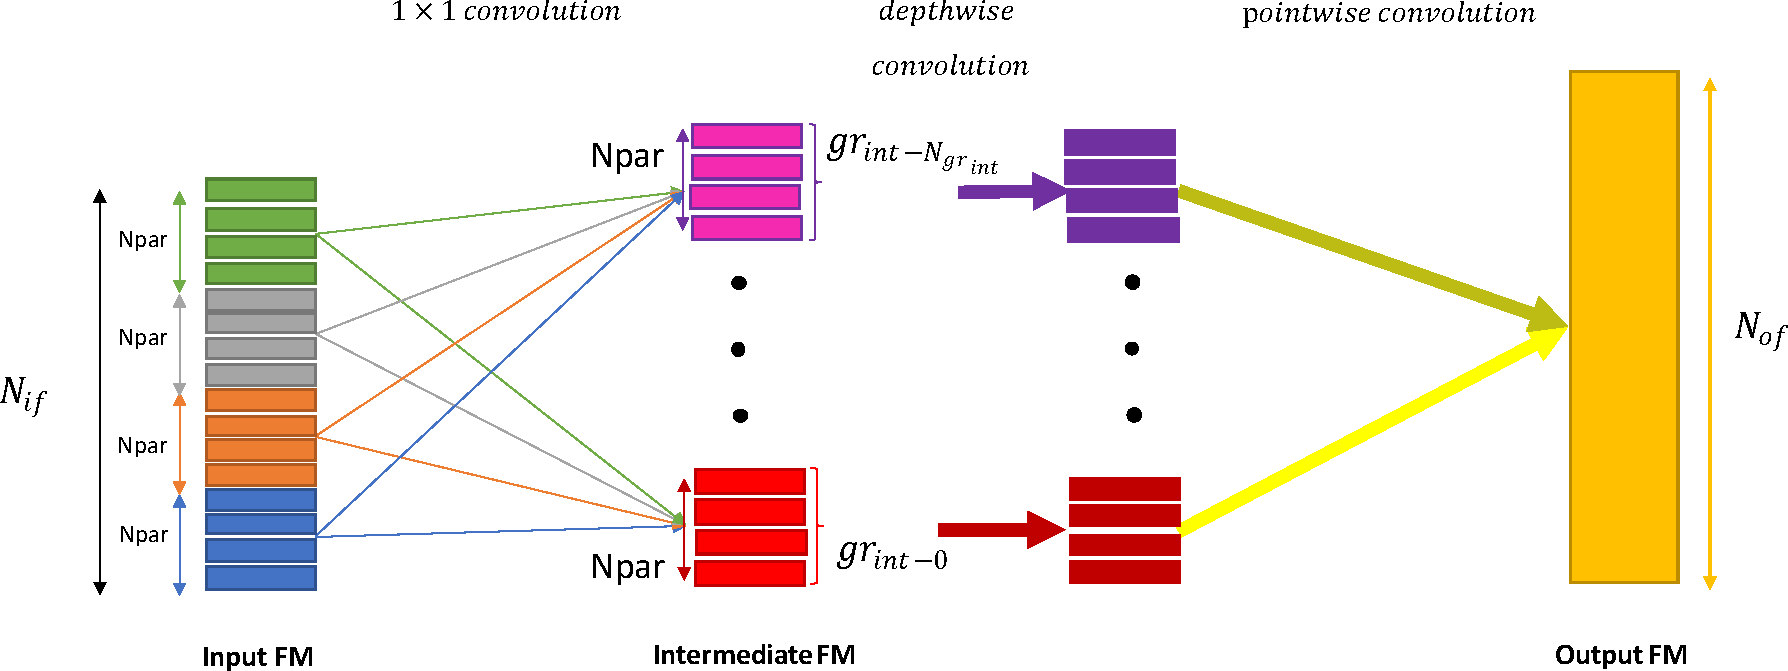
\includegraphics[width=\textwidth]{algo.pdf}
    \caption{Illustration of the algorithm used to perfom the convolutions}
    \label{fig:algo}
\end{figure}

This approach was chosen, instead of producing directly each final output result, to reuse at most the products of the $1 \times 1$ convolution. Indeed, if we aim at directly producing a final output, the $1 \times 1$ convolution has to produce $N_{kx} \times N_{ky} \times N_{ky} \times N_{par}$ intermediate results. When the \acrshort{dsc} has computed the partial sum from this fetching group (for one kernel since we priotize the computation of one final pixel), the old intermediate pixels will be overwritten by next fetching group intermediate pixels, which could have been reused for another pointwise kernel.

We can translate this algorithm into a pseudocode, observed in Algorithm \ref{pseudocode:overal_pseudo_code}, where $group$ (respect. $group_{int}$) is the index of fetching group in the input \acrshort{fm} (resp. intermediate \acrshort{fm}) and $Ngr_{int} = \left\lceil \frac{N_{if} \times t}{N_{par}} \right\rceil$ is the number of intermediate fetching groups. We can now detail how each convolution is going to be performed:
%
\begin{algorithm}[H]
    \centering
    \begin{algorithmic}
        \For{$group_{int}:=0$; $group_{int} < Ngr_{int}$; $group_{int}++$}
            \State{$1 \times 1$ convolution ($group_{int}$)}
            \State{DSC($group_{int}$);}
        \EndFor
    \end{algorithmic}
    \caption{Pseudocode of the algorithm}
    \label{pseudocode:overal_pseudo_code}
\end{algorithm}
%
\begin{enumerate}
    \item \textbf{$1 \times 1$ convolution}: We must fetch the $N_{par}$ kernels corresponding to the \acrshort{dsc} fetching group $group_{int}$. Indeed, the \acrshort{dsc} needs to fetch $N_{par}$ channels of the intermediate \acrshort{fm} (each kernel produces one channel). Then we can perform the convolution with the input \acrshort{fm}. As described in Section \ref{subs:2dconv}, the kernel acts as a sliding window on the input \acrshort{fm}. For each pixel at position $(ix, iy)$, the convolution loads iteratively each weight and pixel fetching group in the channel-axis. For each fetching group $group \leq N_{group}$, the convolution is performed by multiplying each non-pruned weight with its corresponding pixel and accumulates the multiplication with the result of the previous group. The process is finished when the $N_{par}$ intermediate \acrshort{fm} channels have been produced (of size $N_{ix} \times N_{iy}$). The corresponding pseudocode is found in Algorithm \ref{pseudocode:c11} and the process is shown in Figure \ref{fig:algo_11conv}.
    \begin{algorithm}[H]
        \centering
        \begin{algorithmic}
            \For{$int_{f}:=0$; $int_{f} < N_{par}$; $int_{f}++$} \Comment{Loop 3}
                \For{$int_{x}:=0$; $int_{x} < N_{ix}$; $int_{x}++$} \Comment{Loop 2}
                    \For{$int_{y}:=0$; $int_{y} < N_{iy}$; $int_{y}++$} \Comment{Loop 2}
                        \For{$group:=0$; $group < N_{gr}$; $group++$} \Comment{Loop 1}
                            \For{$i_f:=0$; $i_f < N_{np}$; $i_f++$} \Comment{Unrolled}
                                \State{$wgt$  = $filter_{1 \times 1}$[$group_{int} \times N_{par} + int_f$][$group \times N_{np} + i_f$]}
                                \State{$acti$  = $FMI_{I}$[$wgt[pos] + group \times N_{par}$][$int_y$][$int_x$]}
                                \State{FM$_{int}$[$group_{int} \times N_{par} + int_f$][$int_y$][$int_x$]  += $acti \times wgt[val]$}
                            \EndFor
                        \EndFor
                    \EndFor
                \EndFor
            \EndFor
        \end{algorithmic}
        \caption{Sparse $1 \times 1$ convolution pseudocode}
        \label{pseudocode:c11}
    \end{algorithm}
    %
    \begin{figure}[H]
        \centering
        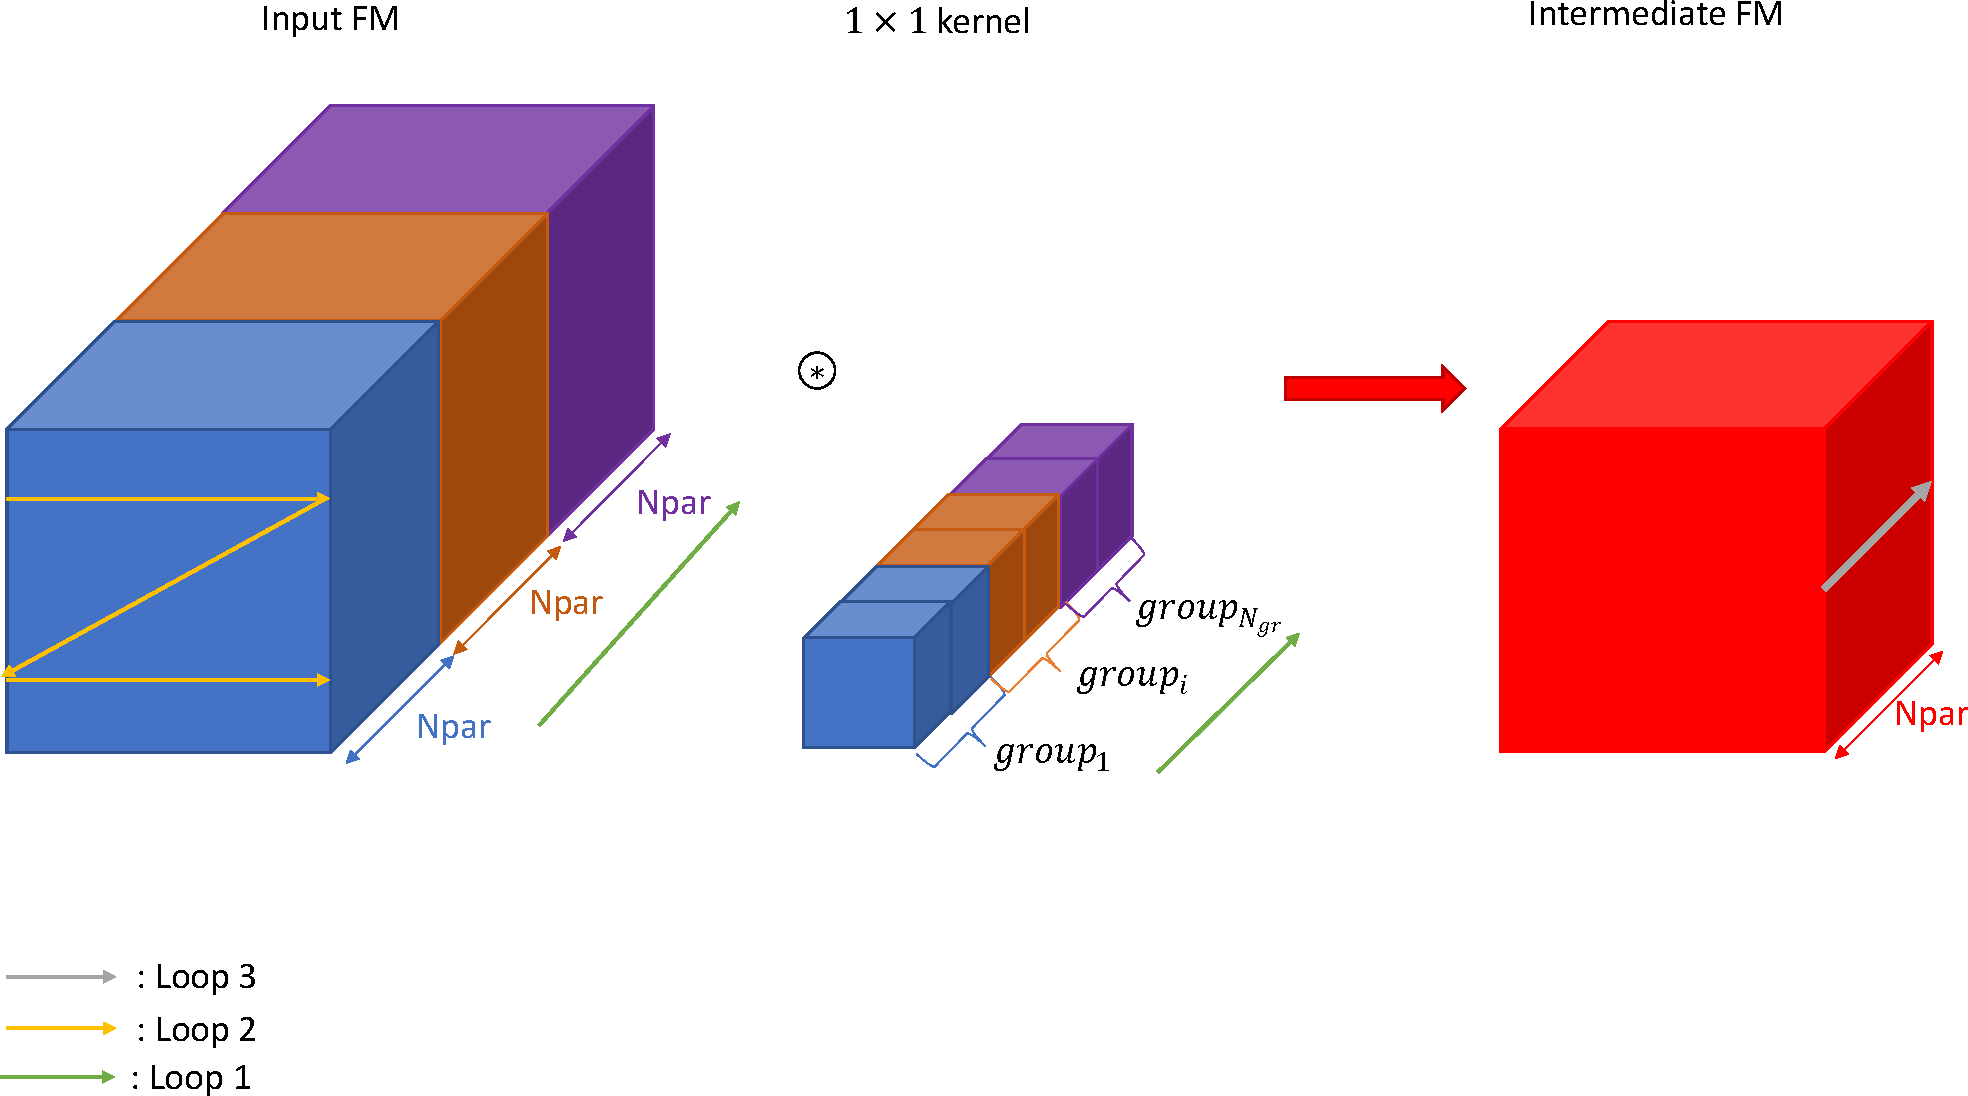
\includegraphics[width=0.75\linewidth]{algo_c11.pdf}
        \caption{Representation of the sparse $1 \times 1$ convolution}
        \label{fig:algo_11conv}
    \end{figure}
    %
    \item \textbf{\acrshort{dsc}} Once the $1 \times 1$ convolution has produced the next $N_{par}$ intermediate \acrshort{fm} channels, we can do the depthwise convolution with these channels. The depthwise convolution first computes the 2D convolution of each of the intermediate \acrshort{fm} channel. Afterwards, we can load the corresponding weight fetching group in each of the pointwise filters. We can compute the partial convolution for each of the output \acrshort{fm}, and each partial result is summed with its corresponding previous partial result. If we do the previous step for every intermediate fetching group, the output \acrshort{fm} is computed. The corresponding pseudocode is found in Algorithm \ref{pseudocode:dsc} and the process is shown in Figure \ref{fig:algo_dsc}. We note that we have to add padding pixels to the intermediate \acrshort{fm} since spatial dimensions are only reduced using stride $S$ (see Section \ref{subs:2dconv}).
    %
    \begin{algorithm}[H]
        \centering
        \begin{algorithmic}
            \For{$o_{y}:=0$; $o_{y} < N_{oy}$; $o_{y}++$} \Comment{Loop 4}
                \For{$o_{x}:=0$; $o_{x} < N_{ox}$; $o_{x}++$} \Comment{Loop 4}
                    \State{\% Depthwise convolution}
                    \For{$int_{f}:=0$; $int_{f} < N_{par}$; $int_{f}++$} \Comment{Loop 3}
                        \For{$k_{y}:=0$; $k_{y} < N_{ky}$; $k_{y}++$} \Comment{Loop 2}
                            \For{$k_{x}:=0$; $k_{x} < N_{kx}$; $k_{x}++$} \Comment{Loop 2}
                                    \State{FM$_{Dw}$[$group_{int} \times N_{par} + int_f$][$o_y$][$o_x$]  += }
                                    \State{FM$_{int}$[$group_{int} \times N_{par} + int_f$][$o_{y} \times S + k_{y}$][$o_{x} \times S + k_{x}$] $\times$} \State{kernel$_{dw}$[$group_{int} \times N_{par} + int_f$][$k_{y}$][$k_{x}$]}
                            \EndFor
                        \EndFor
                    \EndFor
                    \State{\% Pointwise convolution}
                    \For{$o_f:=0$; $o_f < N_{of}$; $of++$} \Comment{Loop 1}
                        \For{$i_f:=0$; $i_f < N_{np}$; $i_f++$} \Comment{Unrolled}
                            \State{$wgt$  = $filter_{Pw}$[$o_f$][$group_{int} \times N_{np} + i_f$]}
                            \State{$acti$  = $FMI_{Dw}$[$wgt[pos] + group_{int} \times N_{par}$][$o_y$][$o_x$]}
                            \State{FM$_{o}$[$o_f$][$o_y$][$o_x$] += $acti \times wgt[val]$}
                        \EndFor
                    \EndFor
                \EndFor
            \EndFor
        \end{algorithmic}
        \caption{Sparse \acrshort{dsc} convolution pseudocode}
        \label{pseudocode:dsc}
    \end{algorithm}
    %
    \begin{figure}[H]
        \centering
        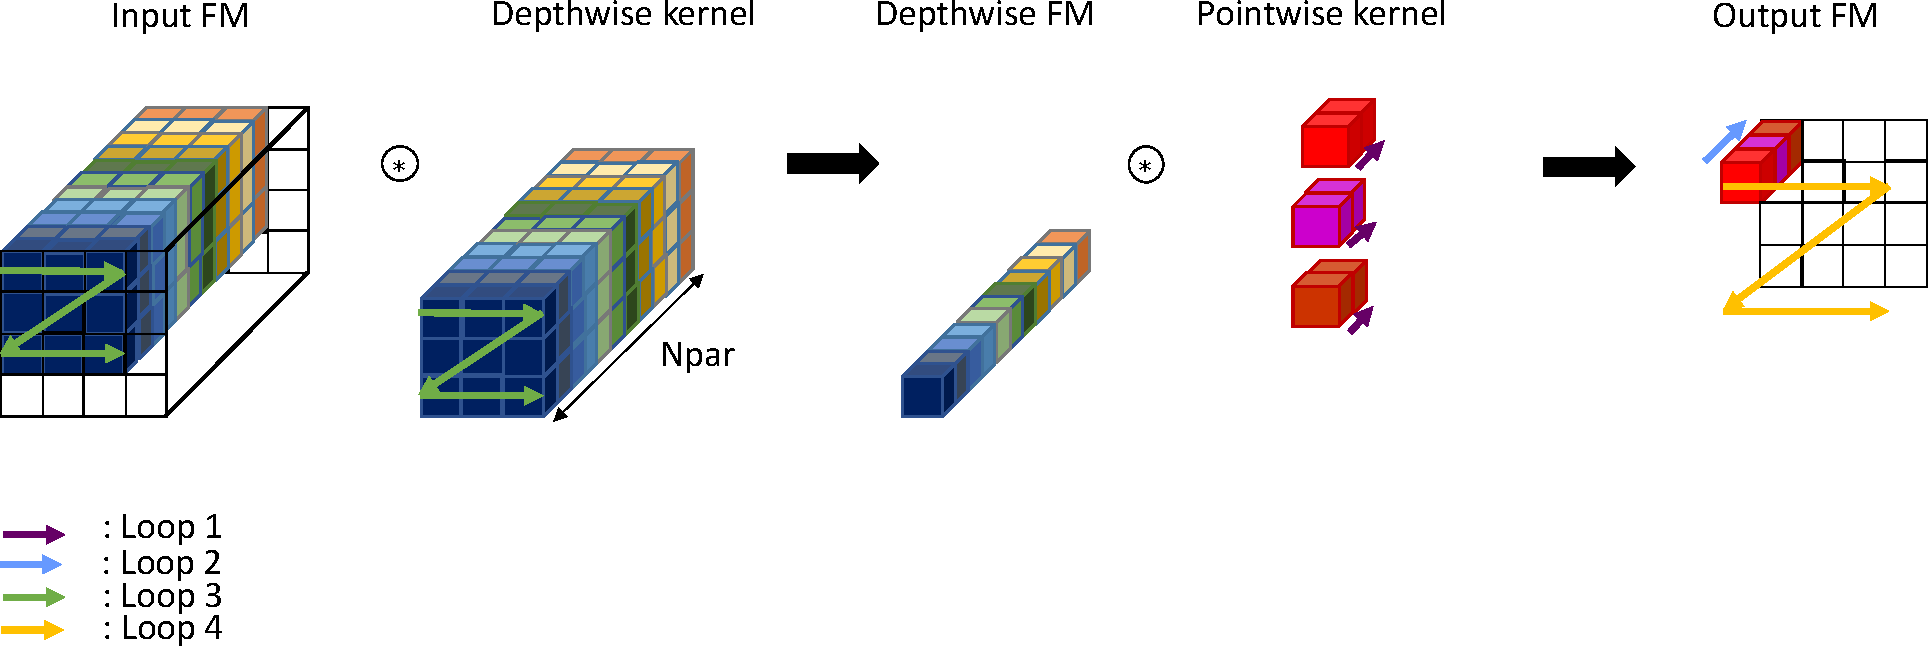
\includegraphics[width=\linewidth]{algo_dsc.pdf}
        \caption{Representation of the sparse \acrshort{dsc} convolution}
        \label{fig:algo_dsc}
    \end{figure}
\end{enumerate}
%
\subsection{Loop analysis}
%
We determined how the convolutions are going to be performed. Therefore, we can define how it will be implemented on \acrshort{fpga}. As explained in Section \ref{sec:opti_dataflow}, the \acrshort{cnn} inference is executed in three steps:
%
\begin{enumerate}
    \item The \acrshort{fpga} loads a tile of the data from the external memory into the on-chip memory.
    \item The \acrshort{pe}s of the \acrshort{fpga} fetch data from the on-chip memory, use them to perform convolution, and store the computed result into the on-chip memory.
    \item Once the tile of output results is produced, it is stored into the external memory. Either the \acrshort{fpga} loads the next tile and restarts the previous steps, either it stops if the last tile of data has been convolved.
\end{enumerate}
%
If we look at Algorithm \ref{pseudocode:c11} and \ref{pseudocode:dsc}, each convolution is implemented with various levels of loop, named \textbf{convolution loops}. To optimize these operations, tree main loop optimization techniques can be used, as presented in Section \ref{sec:opti_dataflow}: loop tiling, loop unrolling, and loop interchange. Those loop optimization techniques include hardware design parameters that define the acceleration factor and hardware footprint \cite{ma_optimizing_2018}. Therefore, we have to analyse the convolution loops in order to find the optimal tiling, unrolling and loop interchange parameters. We applied the same methodology as \textcite{ma_optimizing_2018}. However, as they studied the standard convolution, in this work we adapted it to the proposed sparse \acrshort{dsc}.\cite{ma_optimizing_2018}

\textcite{ma_optimizing_2018} identified design objectives to optimize the convolution operation. These following design objectives should be minimized:
%
\begin{itemize}
    \item Partial sum storage.
    \item On-chip memory accesses and data reutilisation.
    \item Off-chip memory accesses.
\end{itemize}
%
We will try to minimize them for both $1 \times 1$ and depthwise separable convolution.
%
\subsubsection{Hardware design parameters}
%
Before analyzing the design objectives, we must first define what are the different tiling and unrolling parameters for each convolution. Table \ref{tab:param_c11} and Table \ref{tab:param_dsc} defines the different dimensions of the volumes and the corresponding hardware design parameters.

\textbf{$1 \times 1$ convolution}: the $1 \times 1$ convolution is composed of three convolution loops (the fourth loop is fully-unrolled according to the algorithm). During Loop-1, we get each fetching group and we do the convolution between them. Loop-1 is determined by the number of input and weight fetching groups (they are the same since otherwise there would be misalignement). The purpose of Loop-1 is to compute the output final result of the convolution. Loop-2 slides spatially the kernel over the input \acrshort{fm} to produce one channel of the intermediate \acrshort{fm}. Since the spatial size of each kernel is $1 \times 1$, there is no spatial reduction between the input and intermediate \acrshort{fm}. The purpose of Loop-3 is to choose which of the required $N_{par}$ intermediate \acrshort{fm} channels is produced.
%
\begin{table}[H]
    \centering
    \begin{tabular}{c|c|c|c}
    \hline \hline
    & \makecell{\# of weight \\ and input \\ fetching group} & \makecell{Input \acrshort{fm} \& \\ intermediate \acrshort{fm} \\ Spatial Axis} & \makecell{intermediate \acrshort{fm} \\ channels} \\
    \hline
    Convolution Loops & Loop-1 & Loop-2 & Loop-3 \\
    Convolution Dimensions & $N_{gr}$ & $N_{ix}$,$N_{iy}$ & $N_{par}$ \\
    Loop Tiling            & $T_{gr}$ & $T_{ix}$,$T_{iy}$ & $T_{intf}$ \\
    Loop Unrolling         & $P_{gr}$ & $P_{ix}$,$P_{iy}$ & $P_{intf}$ \\
    \hline \hline
    \end{tabular}
    \caption{$1 \times 1$ convolution loop dimensions and hardware design variables, inspired by \cite{ma_optimizing_2018}}
    \label{tab:param_c11}
\end{table}
%
\textbf{\acrshort{dsc}}: the \acrshort{dsc} is composed of four convolution loops. Two loops are specific to the depthwise convolution, one to the pointwise convolution and one loop is shared between the two convolutions. As presented in Section \ref{subsec:mbnv2-pr}, the pointwise convolution uses the results of the depthwise convolution to produce $N_{of}$ partial results in order to avoid reperforming the same $1 \times 1$ and depthwise convolutions. Loop-1 therefore aims at looping over the output channels. The depthwise convolution is composed of two loops. Loop-2 performs the 2D convolution between the input channel and the corresponding kernel and Loop-3 loops over the input channel. Finally, Loop-4 is the one that selects which output pixels to compute and fetches the associated input pixels chunk of data from the on-chip memory.
%
\begin{table}[H]
    \centering
    \begin{tabular}{c|c|c|c|c|c}
    \hline \hline
    & \makecell{Output \acrshort{fm} \\ channels} & \makecell{Pointwise \\ kernel size} & \makecell{Intermediate\\\acrshort{fm} channels} & \makecell{Intermediate \acrshort{fm} \\ Spatial Axis} & \makecell{Output \acrshort{fm} \\ Spatial Axis} \\
    \hline
    \makecell{Convolution \\ Loops}      & Loop-1   & Loop-2            & Loop-3     & Loop-4            & Loop-4 \\
    \makecell{Convolution \\ Dimensions} & $N_{of}$ & $N_{kx}$,$N_{ky}$ & $N_{par}$  & $N_{ix}$,$N_{iy}$ & $N_{ox}$,$N_{oy}$\\
    \makecell{Loop \\ Tiling}            & $T_{of}$ & $T_{kx}$,$T_{ky}$ & $T_{intf-dw}$ & $T_{ix}$,$T_{iy}$ & $T_{ox}$,$T_{oy}$\\
    \makecell{Loop \\ Unrolling}         & $P_{of}$ & $P_{kx}$,$P_{ky}$ & $P_{intf-dw}$ & $P_{ix}$,$P_{iy}$ & $P_{ox}$,$P_{oy}$\\
    \hline \hline
    \end{tabular}
    \caption{\acrshort{dsc} loop dimensions and hardware design variables, inspired by \cite{ma_optimizing_2018}}
    \label{tab:param_dsc}
\end{table}
%
\subsubsection{Partial Sum Storage}
%
\textbf{$1 \times 1$ convolution}: on order to minimize the partial sum storage, we have to keep all partial results in the registers. If we store those partial results into the on-chip or off-chip memory, it would result in accesses that are less efficiency in terms of energy consumption and latency. The optimal solution would be to fully unroll Loop-1. However, two problems arise. First, since the \acrshort{fpga} has constrained resources, it could not be feasible on the target platform. Second, the number of fetching groups vary accross the layers since it depends on the number of input channels ($N_{gr} = \frac{N_{if}}{N_{par}}$). We should adapt the unrolling parameter $P_{gr}$ to the worst case and there would be inefficiency problems. Indeed, if $N_{gr} < P_{gr}$, some \acrshort{pe} would not be used. A better solution would be to fully buffer each fetching group and keep the partial results in the registers. Therefore, we should compute Loop-1 first (otherwise some results would be stored in the on-chip memory).
In summary, the number of partial sums is determined by the number of $1 \times 1$ convolution \acrshort{pe}s in parallel, as shown in Equation \eqref{eq:psum_c11}. Each $1 \times 1$ convolution \acrshort{pe} can operate in parallel $P_{gr}$ fetching groups. To minimize the storage of partial sum, we should add the following constraint $T_{gr} = N_{gr}$. Moreover, the ratio of $P_{gr}$ to each $N_{gr}$ of the network should be an integer to avoid these inefficiency problems.
%
\begin{equation}
    \# psum_{1 \times 1} = P_{ix} \times P_{iy} \times P_{intf}
    \label{eq:psum_c11}
\end{equation}

\textbf{\acrshort{dsc}}: we can find two kinds of partial sums: the partial depthwise results and the partial output results. According to the proposed algorithm, we can not keep the partial output in the registers since we produce from each intermediate fetching group every possible partial output results. It means that we must keep the tile of output \acrshort{fm} in the on-chip memory as partial results, as illustrated in Equation \eqref{eq:psum_o_dsc}. Since the kernel size is small and constant accross the network, we can fully unroll Loop-2 and set $P_{kx} = T_{kx} = N_{kx}, P_{ky} = T_{ky} = N_{ky}$. This approach was also chosen by \textcite{motamedi_placid_2017}. Since the fetching group size $N_{par}$ is up to the programmer, we can also fully unroll Loop-3 $P_{intf-dw} = T_{intf-dw} = N_{par}$. As the depthwise convolution is fully unrolled, we can determine the number of depthwise partial sums using equation \eqref{eq:psum_dw_dsc}.
%
\begin{equation}
    \# psum_{DSC_{PW}} = T_{ox} \times T_{oy} \times T_{of}
    \label{eq:psum_o_dsc}
\end{equation}
%
\begin{equation}
    \# psum_{DSC_{DW}} = N_{kx} \times N_{ky} \times N_{par}
    \label{eq:psum_dw_dsc}
\end{equation}
%
\subsubsection{On-chip memory accesses}
%
According to \textcite{ma_optimizing_2018}, the number of on-chip accesses is determined by Equation \eqref{eq:onchipaccess}, where $\#read_{px}$ (resp. $\#read_{wg}$) is the number of reads in the on-chip memory accesses for input pixel (resp. weight), $\#read\_write\_psum$ is the number of write and read accesses if we store partial sum in the on-chip memory, and  $\#write\_px$ is the number of accesses to write the output results (which is equal to the number of output pixels). Therefore, to reduce on-chip memory accesses, we mus limit partial sums stored in on-chip memory and limit the number of reads.
The number of reads can be reduced by reusing the data in the registers, and can be expressed using Equation \ref{eq:read_on_px} and \ref{eq:read_on_wg} \cite{ma_optimizing_2018}, where $N_{op}$ is the total number of operations in a convolution. We can analyze for each convolution $Data\_Reuse_{px}$ and $Data\_Reuse_{wg}$.
%
\begin{multline}
    \#On\_chip\_accesses = \#read_{px} + \#read_{wg} + \\ \#read\_write\_psum + \#write\_px
    \label{eq:onchipaccess}
\end{multline}
%
\begin{equation}
    \#read_{px} = \frac{N_{op}}{Data\_Reuse_{px}}
    \label{eq:read_on_px}
\end{equation}
%
\begin{equation}
    \#read_{wg} = \frac{N_{op}}{Data\_Reuse_{wg}}
    \label{eq:read_on_wg}
\end{equation}

\textbf{$1 \times 1$ convolution}: data reuse should be maximized to limit the number of on-chip memory accesses which are less efficient than register accesses. \textcite{ma_optimizing_2018} define two kinds of data reutilisation: spatial reuse (how many data are reused in one cycle) and temporal reuse (if a data can be reused in more than one cycle). Temporal data reuse is only possible if we compute Loop-2 first (we keep the same kernel for the pixels of a channel). However, since we compute Loop-1 first, this is not possible. To increase spatial data reuse, we must increase the parallelization and so the unrolling parameters, as illustrated in Equation \eqref{eq:px-d-reu} and \eqref{eq:wg-d-reu}, where $Data\_Reuse_{px}$ (resp. $Data\_Reuse_{wg}$) is the data reuse for input pixels (resp. weight).
%
\begin{equation}
    Data\_Reuse_{px - 1 \times 1} = P_{intf}
    \label{eq:px-d-reu}
\end{equation}
\begin{equation}
    Data\_Reuse_{wg - 1 \times 1} = P_{ix} \times P_{iy}
    \label{eq:wg-d-reu}
\end{equation}

\textbf{\acrshort{dsc}}: Since Loop-3 and Loop-2 are fully unrolled, we have a full temporal data reuse for depthwise weight. The data reuse for pixel and weight for the depthwise convolution can be found in Equation \eqref{eq:px_dw-d-reu} \cite{ma_optimizing_2018} and \eqref{eq:wg_dw-d-reu}. For the pointwise convolution, we can avoid reading input pixels from on-chip memory if we keep the $N_{par}$ results of the depthwise convolution in registers.
Using the same methodology as for \textbf{$1 \times 1$ convolution}, the weight data reuse can be expressed using Equation \eqref{eq:wg_pw-d-reu}
%
\begin{equation}
    Data\_Reuse_{px - dsc} = \frac{N_{kx} \times N_{ky} \times N_{par} \times P_{intx} \times P_{inty}}{\left( \left( P_{intx} - 1 \right)S + N_{kx} \right) \times \left( \left( P_{inty} - 1 \right)S + N_{ky} \right)}
    \label{eq:px_dw-d-reu}
\end{equation}
\begin{equation}
    Data\_Reuse_{wg-dw} = N_{kx} \times N_{ky} \times N_{par}
    \label{eq:wg_dw-d-reu}
\end{equation}
\begin{equation}
    Data\_Reuse_{wg-pw} = P_{ox} \times P_{oy}
    \label{eq:wg_pw-d-reu}
\end{equation}
%
\subsubsection{Off-chip memory accesses}
%
In the model presented in Section \ref{subsec:loopopti}, as the on-chip memory is not large enough to store the whole \acrshort{cnn} size, this one is stored in an external memory. However, accesses to the external memory are more expensive in terms of latency and energy. Therefore, we should limit the number of off-chip memory accesses per pixel and weight. Instead, we tile the weights and input \acrshort{fm} that we store in the on-chip memory. Once the tile has been fully used, we can load the next tile until the convolution is done.

Since we store every pixel fetching group in the on-chip memory, each pixel is loaded only once from the external memory. However, thanks to padding and the 2D convolution, the input \acrshort{fm} tile can be expressed as Equation \eqref{eq:tileo} \cite{ma_optimizing_2018}. If the input \acrshort{fm} tile does not cover the spatial size of the input \acrshort{fm}, some pixels are included in multiple tiles due to the depthwise convolution, as illustrated in Figure \ref{fig:tilei}. Despite this, it does not concern every pixel. Therefore, we can express the number of external memory accesses per pixel as Equation \eqref{eq:dram_px}.
%
\begin{equation}
    T_{ix/iy} = \left( T_{ox/oy} - 1\right) S + P_{kx/ky}
    \label{eq:tileo}
\end{equation}
\begin{equation}
    \#DRAM\_px = 1
    \label{eq:dram_px}
\end{equation}
%
\begin{figure}[H]
    \centering
    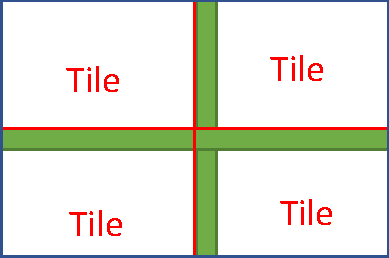
\includegraphics[width=0.6\textwidth]{Tile.pdf}
    \caption{Tiling process on an input \acrshort{fm}, where the green area is the input pixels that would be loaded more than once due to 2D convolution}
    \label{fig:tilei}
\end{figure}
%
If all the weights are not buffered into the on-chip buffer, we have to load from external memory the weight corresponding to the intermediate \acrshort{fm} fetching group. It means that we must fetch each weight everytime a new output tile is produced. Therefore, the number of weight external memory access is expressed as Equation \eqref{eq:dram_wg}.
%
\begin{equation}
    \#DRAM\_px = \frac{N_{ox} \times N_{oy}}{T_{ox} \times T_{oy}}
    \label{eq:dram_wg}
\end{equation}
%
\subsubsection{Summary}
%
After analyzed the convolution loop, we determined the unrolling and tiling hardware design parameters:
\begin{itemize}
    \item Loop interchange: for both convolutions, we do the loops in the given order (first Loop-1, ..., and then Loop-n).
    \item Loop Tiling: as explained previously, the following tiling parameters are set:
    \begin{itemize}
        \item $T_{gr} = N_{gr}$
        \item $T_{intf} = N_{par}$
        \item $T_{intf-dw} = N_{par}$
        \item $T_{of} = N_{of}$
        \item $T_{kx} = N_{kx}$
        \item $T_{ky} = N_{ky}$
    \end{itemize}
    The other tiling parameters should be set as close as $N_{*}$ (depending on the target platform). Moreover, as pointed out by \textcite{ma_optimizing_2018}, the following constraint should be added to avoid inefficiency: \textquote{$T_{*}$ should be a divisor of $N_{*}$}. Indeed, the \acrshort{pe}s are configured to execute a full tile. If the constraint is not satisfied, some \acrshort{pe}s would not be used.
    \item Loop Unrolling: as explained previously, the following unrolling parameters are set:
    \begin{itemize}
        \item $P_{kx} = N_{kx}$
        \item $P_{ky} = N_{ky}$
        \item $P_{intf-dw} = N_{par}$
    \end{itemize}
    The other unrolling parameters should be set as close as $T_{*}$ (depending on the target platform). Moreover, as pointed out by \textcite{ma_optimizing_2018}, the following constraint should be added to avoid inefficiency: \textquote{$P_{*}$ should be a divisor of $T_{*}$}.
\end{itemize}
%% unrolling

%
%
\section{Implementing sparse DSC on FPGA} \label{sec:implementation}
In the previous section, we detailed how to prune $1 \times 1$ kernels, how the bottleneck convolution is computed, and we analyzed the design hardware variables. In this section, we explore how we can implement the chosen design into an \acrshort{fpga}. The hardware design was implemented using SystemVerilog and the corresponding code can be found at this address: 
%
\begin{center}
    \url{https://github.com/ggheysen/UCL-EPL-Master-Thesis-2019-2020}.
\end{center}
%
According to the scope of this thesis, the purpose of the implementation is to verify the fourth and fifth design objectives, namely:
%
\begin{itemize}
    \item The proposed architecture provides a logically correct output.
    \item An increase of the sparsity improves the performance of the architecture.
\end{itemize}
%
Those design objectives are related to the implementation of the inverted residual block with sparse $1 \times 1$ convolution. Therefore, instead of implementing each type of layer of MobileNetV2, we focus only on this one. As those two objectives are independent of the degree of parallelization, it was chosen to set all unrolling parameters to 1. We did not implement the skip connection since it is independent of the pruning scheme. However, as demonstrated by \textcite{bai_cnn_2018, liu_fpga-based_2019}, we can extend the \acrshort{dsc} \acrshort{pe}s to support all kind of layers of MobileNetV2.

First, we start by describing the overall architecture of the accelerator. Then, we detail more precisely each component defined previously. The performance results of the architecture will be discussed in next section.

The architecture is inspired by three works: \textcite{zhu_efficient_2020, kang_accelerator-aware_2020, bai_cnn_2018}.
%
\subsection{Overall architecture} \label{subsec:overal}
%
The overall architecture has been inspired by \textcite{zhu_efficient_2020}. The mains components that compose our \acrshort{fpga}-based architecture are the following:
%
\begin{itemize}
    \item \textbf{External Memory}: it contains the \acrshort{cnn} data and it is where the output \acrshort{fm} will be stored.
    \item \textbf{Main controller}: it synchronizes the different components of the architecture by sending them control signals.
    \item \textbf{\acrfull{dma}}: it handles the read and write requests between the \acrshort{fpga} and the external memory.
    \item \textbf{\acrshort{pe}}: each \acrshort{pe} performs the convolution with weight and pixel fetched from external memory into the on-chip memory. In the architecture, we have two kinds of \acrshort{pe}: $1 \times 1$ convolution \acrshort{pe} and \acrshort{dsc} \acrshort{pe}. Since we have defined that each data is represented using fixed-point number format (see Section \ref{subs:quantization}), the convolution between weights and pixels is done with integer arithmetic.
    \item \textbf{Buffer}: it composes the on-chip memory and contains a tile of data. There are two categories of buffer: \textbf{data buffer} which contains convolution data (pixels and weights) loaded from the external memory, and \textbf{result buffer} which contains partial or final results of the $1 \times 1$ or \acrshort{dsc} convolutions. Our architecture is composed of four data buffers ($FM_{I}$ buffer, $Conv_{1 \times 1}$ buffer, $Conv_{DW}$ buffer, $Conv_{PW}$ buffer) and two result buffers ($FM_{int}$ buffer, $FM_{O}$ buffer).
\end{itemize}
%
An illustration of the overall architecture can be found in Figure \ref{fig:overal_archi}. We should add that every component is synchronous with the clock signal $clk$ and is reset when the $rst$ signal is enabled. For the sake of clarity, this was not included in the drawing.
%
\begin{figure}[H]
    \centering
    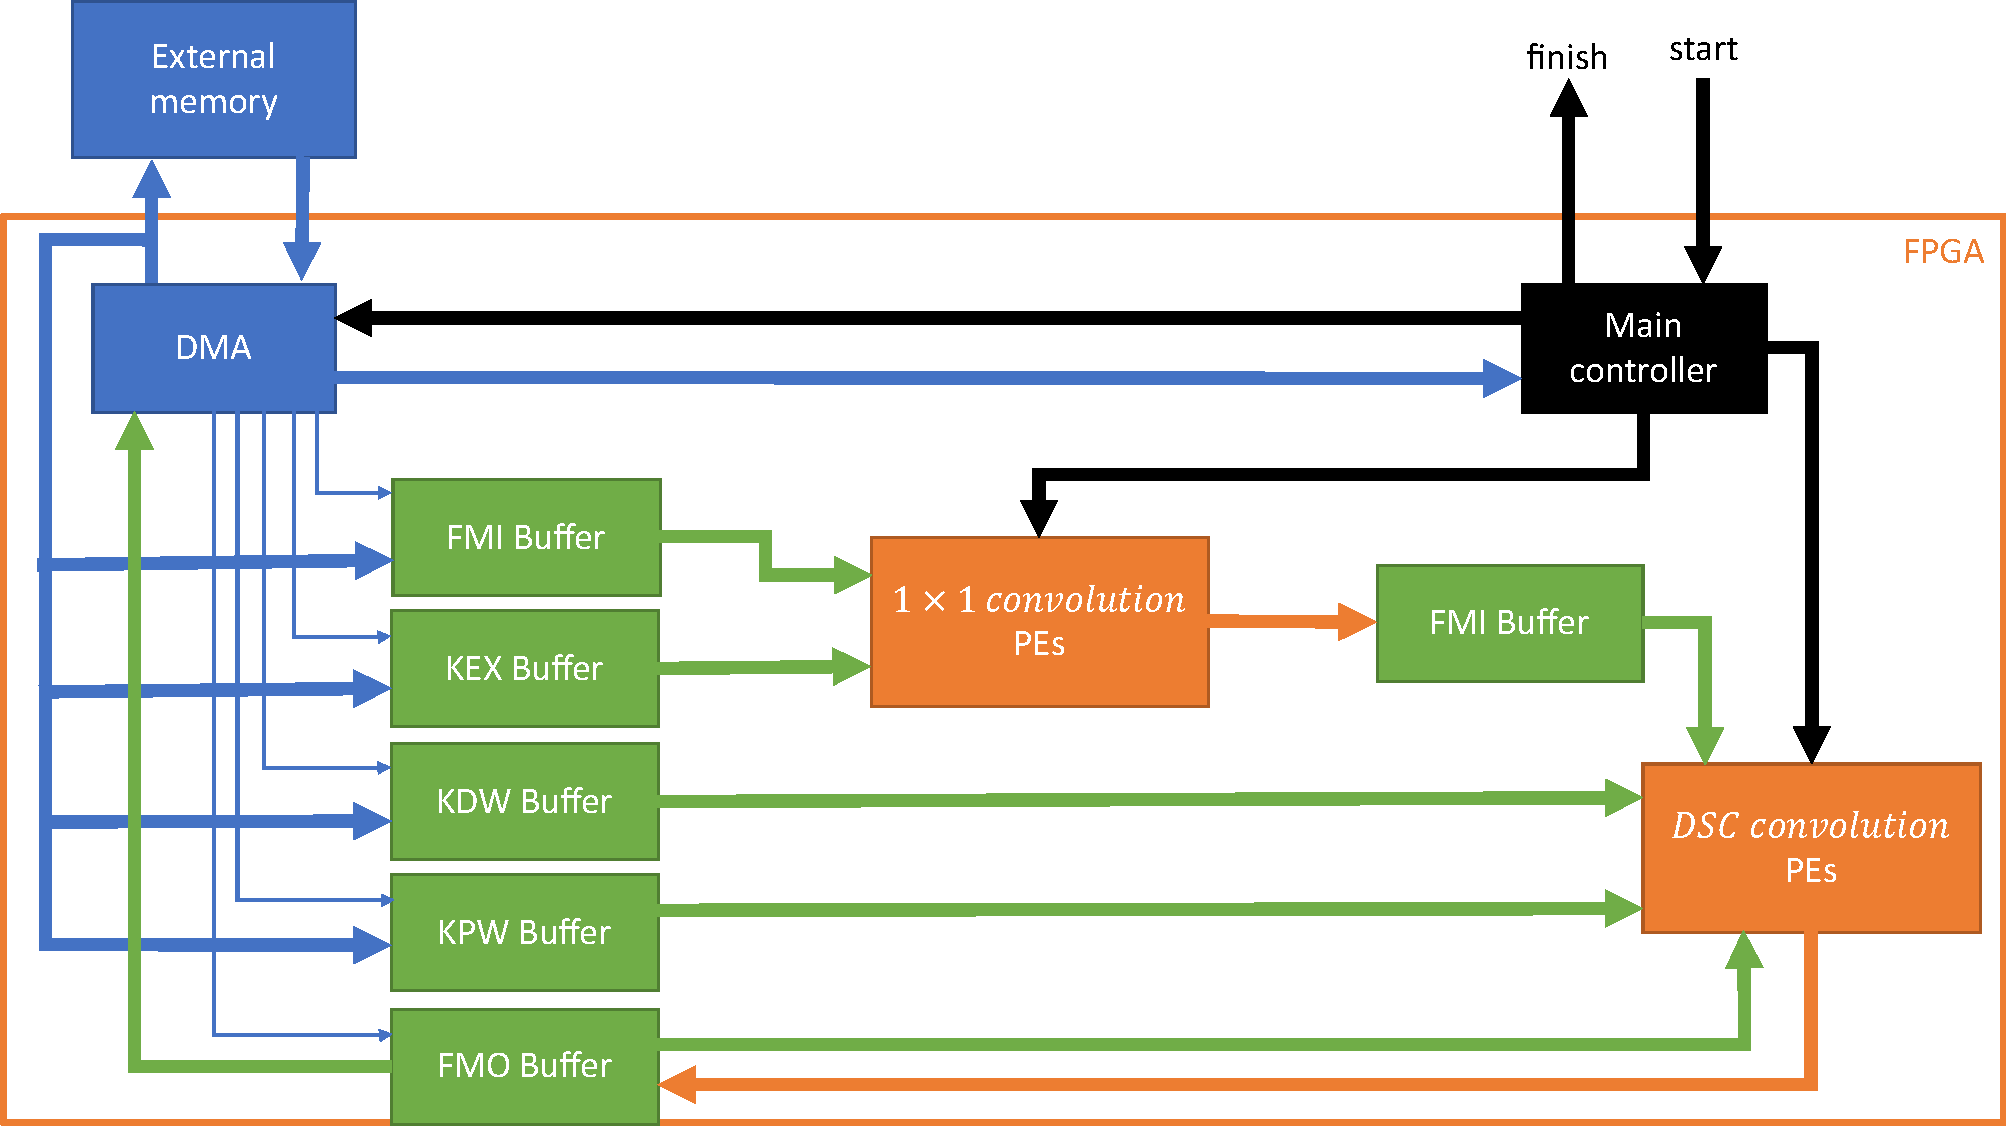
\includegraphics[width=\textwidth]{overal_archi.pdf}
    \caption{overall architecture of the accelerator}
    \label{fig:overal_archi}
\end{figure}
%

We explain more precisely the behavior of each component in the following sections. An exhaustive list of their different input and output signals can be found in Appendix \ref{appendix:sig}.
%
\subsection{External memory} \label{subs:extmem}
%
The external memory is an external component (of the \acrshort{fpga}) that contains all the data required to feed the network (MobileNetV2). Each data stored in a memory can be identified by its address (either external memory or buffer). We can identify 6 types of data:
%
\begin{enumerate}
    \item \textbf{Input \acrshort{fm}}: where the bitwidth required to represent the value of one pixel is equal to $BW_{pixel}$. Channels are stored one by one, and the content of one channel is stored line by line. For example, the memory address of the pixel at position $\left(ix, iy, if\right)$ can be expressed using Equation \eqref{eq:addr_fmi}.
    \begin{equation}
        address_{FM_{I}}(ix, iy, if) = ix + iy \times N_{ix} + if \times N_{ix} \times N_{iy}
        \label{eq:addr_fmi}
    \end{equation}
    \item \textbf{Output \acrshort{fm}}: the output \acrshort{fm} is stored in the same manner as the input \acrshort{fm}. We should add that the output \acrshort{fm} of one layer becomes the input \acrshort{fm} of the next layer. Therefore, the addresses where the output \acrshort{fm} pixels are stored become the addresses of the input \acrshort{fm} of the next layer and inversely.
    %
    \item \textbf{$1 \times 1$ kernels}: the weights of each $1 \times 1$ convolution (bottleneck layers and $1 \times 1$ convolution layers), where $BW_{weight}$ is the number of bits to represent the value of a weight and $log_2(N_{par})$ the number of bits to represent its position. Each $1 \times 1$ filter is stored kernel by kernel, and each kernel is stored weight by weight. For example, the memory address of the weight $x$ in fetching group \textquote{$group$} of kernel $f$ can be expressed using Equation \eqref{eq:addr_c11}.
    %
    \begin{equation}
        address_{K_{EX}}(kx, group, kf) = kx + group \times N_{np} + kf \times N_{np} \times N_{gr}
        \label{eq:addr_c11}
    \end{equation}
    %
    \item \textbf{Depthwise kernels}: the depthwise kernels, where the bitwidth representing one weight is equal to $BW_{weight}$. Channels are stored one by one, and the content of one channel is stored line by line. For example, the memory address of the weigth at position $\left(kx, ky, kf\right)$ can be expressed using Equation \eqref{eq:addr_dw}.
    %
    \begin{equation}
        address_{K_{DW}}(kx, ky, kf) = kx + ky \times N_{kx} + kf \times N_{kx} \times N_{ky}
        \label{eq:addr_dw}
    \end{equation}
    %
    \item \textbf{Pointwise kernels}: the kernels of the pointwise convolution. The weights are stored in the same manner as for the $1 \times 1$ filter.
    %
    \item \textbf{Standard convolution kernels}: since the first layer of MobileNetV2 is a standard convolution \cite{sandler_mobilenetv2_2018}, the weights must be also stored in the external memory, in the same manner as the depthwise filter.
\end{enumerate}

An offset for each type of data is added to the computation of the address to avoid that one address is shared between multiple data. As a result, before executing one layer, the main controller must have the following information, labelled as \textbf{Layer information}:
%
\begin{enumerate}
    \item $\boldsymbol{N_{ix}}$ and $\boldsymbol{N_{iy}}$: the spatial dimensions of the input \acrshort{fm}. Since $N_{ix}, N_{iy} \leq 224$ \cite{sandler_mobilenetv2_2018}, we can use 8 bits to represent them.
    \item $\boldsymbol{N_{if}}$ and $\boldsymbol{N_{of}}$: the number of channels of the input  and output \acrshort{fm}. Since $N_{if}, N_{of} \leq 1280$ \cite{sandler_mobilenetv2_2018}, we can use 11 bits to represent them.
    \item $\boldsymbol{t}$: the expansion factor of the $1 \times 1$ convolution. Since $t \leq 6$ \cite{sandler_mobilenetv2_2018}, we can use 3 bits to represent it.
    \item $\boldsymbol{S}$: the value of the stride. Since $S$ can be either 1 or 0 \cite{sandler_mobilenetv2_2018}, we can use 1 bit to represent it.
    \item $\boldsymbol{N_{gr}}$ and $\boldsymbol{N_{gr-int}}$: the number of fetching groups for the $1 \times 1$ convolution and the \acrshort{dsc}. Since the largest value possible for both parameters is the maximum $N_{if}$ ($N_{par} = 1$), we can use 11 bits to represent them.
    \item $\boldsymbol{Layer}$: to tell the main controller which layer is going to be executed. Since there are 4 kinds of layers in MobileNetV2 \cite{sandler_mobilenetv2_2018}, we use 2 bits to represent it. However this was not included in the design because only the bottleneck convolution was implemented.
    \item \textbf{Offsets}: the offset of the different data types must be transfered to the \acrshort{dma} in order to correctly compute the address of the required data. The number of bits required to represent one offset is the bitwidth of the address of the external memory.
\end{enumerate}
%
As a consequence, those layer information are also stored in the external memory. The overall structure of the external memory can be found in Figure \ref{fig:overal_mem}.
%
\begin{figure}[H]
    \centering
    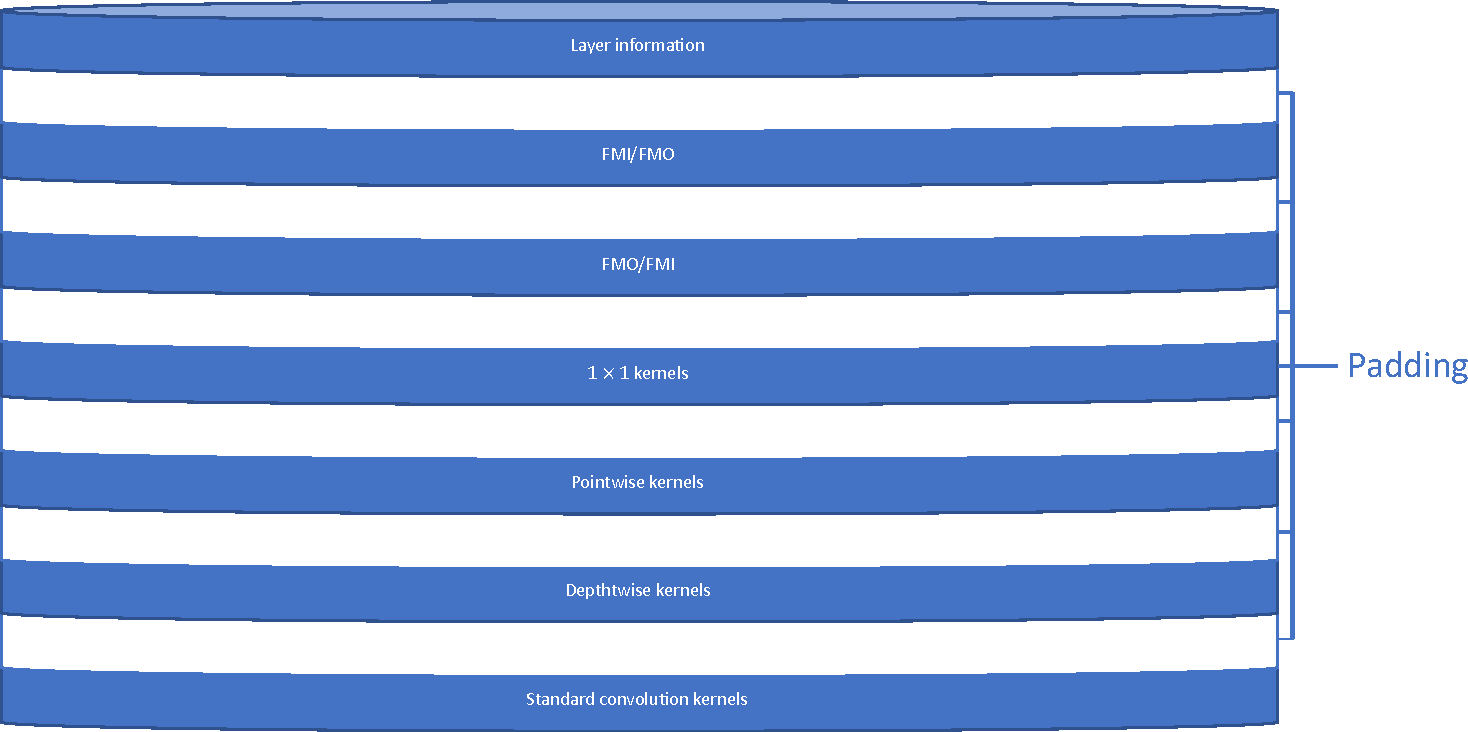
\includegraphics[width=0.75\textwidth]{overal_mem.pdf}
    \caption{overall structure of the external memory}
    \label{fig:overal_mem}
\end{figure}
%
We can now evaluate the total memory size required to hold the \acrshort{cnn}. Since this depends on the pruning parameters, we compute the upper-bound of memory required ($\alpha = 1, N_{par} = N_{if-max}$). For the same reason, we also set the memory required to store each filter or \acrshort{fm} as the memory usage of the largest element of the same type accross all layers of the network. Moreover, according to \cite{noauthor_cyclone_2018}, the maximum external memory size for Cyclone V supported is $4GB$, and hence the maximum bitwidth of the offset is $32 \ bits$. Similarly, the maximum $BW_{pixel}$ and $BW_{weight}$ is equal to $32 \ bits$.

As a result, the memory usage of the network depending on the bitwidth used to represent each pixel and weight is expressed in Equation \eqref{eq:max-extmem}.
The curve representing the maximal external memory required can be found in Figure \ref{fig:max-mem}. We can conclude that we need an external memory size of at least 70 $MB$, which is smaller than the maximal external memory of Cyclone V \acrshort{fpga} ($4 GB$)
%
\begin{align}
    \# layers_{tot} &= 21 \\
    \# layers_{standard-conv} &= 1 \\
    \# layers_{bottleneck-conv} &= 17 \\
    \# layers_{1-1-conv} &= 2 \\
    BW_{layer_{information}} &= 258 \text{ bits} \\
    Max\_FMI &= 112 \times 112 \times 32 = 401408 \\
    Max\_FMO &= Max\_FMI \\
    Max\_K11\_filter &= 320 \times 1280 = 409600 \\
    Max\_KDW\_filter &= 3 \times 3 \times 6 \times 160 = 8640\\
    Max\_KPW\_filter &= 6 \times 160 \times 320 = 307200 \\
    Max\_KSC\_filter &= 3 \times 3 \times 32 = 288
\end{align}
%
\begin{equation}
    \begin{split}
        Max\_Mem = &\left(\# layers_{tot} \times BW_{layer_{information}} \right) \\
        &+ \left( Max\_FMI \times BW_{pixel} \right) \\
        &+ \left( Max\_FMO \times BW_{pixel} \right) \\
        &+ \left( \# layers_{standard-conv} \times Max\_KSC\_filter \times BW_{weight} \right) \\
        &+ \left( \# layers_{bottleneck-conv} \times Max\_KDW\_filter \times BW_{weight} \right)\\
        &+ \left( \# layers_{bottleneck-conv} \times Max\_KPW\_filter \times \alpha \times(BW_{weight} + log_2(N_{par})) \right)\\
        &+ ( \left(\# layers_{bottleneck-conv} + \# layers_{1-1-conv}\right) \times \\
        & \ \ \alpha \times Max\_K11\_filter \times  (BW_{weight} + log_2(N_{par})) )
    \end{split}
\label{eq:max-extmem}
\end{equation}
%
\begin{figure}[H]
    \centering
    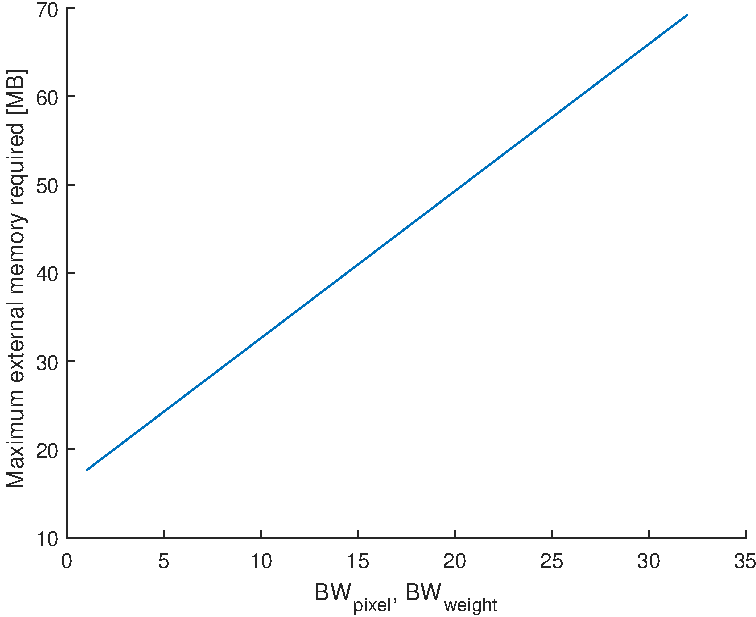
\includegraphics[width=0.75\textwidth]{maxmem.pdf}
    \caption{Maximum external memory required in $MB$ in relation with the bitwidth of each data $BW_{pixel}$ and $BW_{weight}$}
    \label{fig:max-mem}
\end{figure}
%
The maximum memory required can be reduced with pruning. For example, by modifying Equation \eqref{eq:max-extmem}, with $N_{par} = 8, N_{np} = 4$, and $BW_{weight} = BW_{pixel} = 16$, the total memory required is equal to 16.54 $MB$.
%
\subsection{Main controller}
%
The role of the main controller is to synchronize the different components of the architecture (except the memory components). Therefore, each component is a \textquote{slave} that stays in an idle state until the main controller wakes up one of them to perform a particular operation.

To wake up a component, the main controller sends it a starting signal $s_{*}$ and optionnaly additional information about the operation to perform. Afterwards, the main controller remains idle, waiting for the component to terminate its operation. Once the component has completed its task, it sends a finishing signal $f_{*}$ to the main controller.

The main controller remains in an idle state until it receives a starting signal indicating that the external memory contains all data to perform a bottleneck convolution. I have implemented the main controller to compute one bottleneck convolution, but its architecture could be extended to iterate through all the layers of the network.

%
\begin{figure}
    \centering
    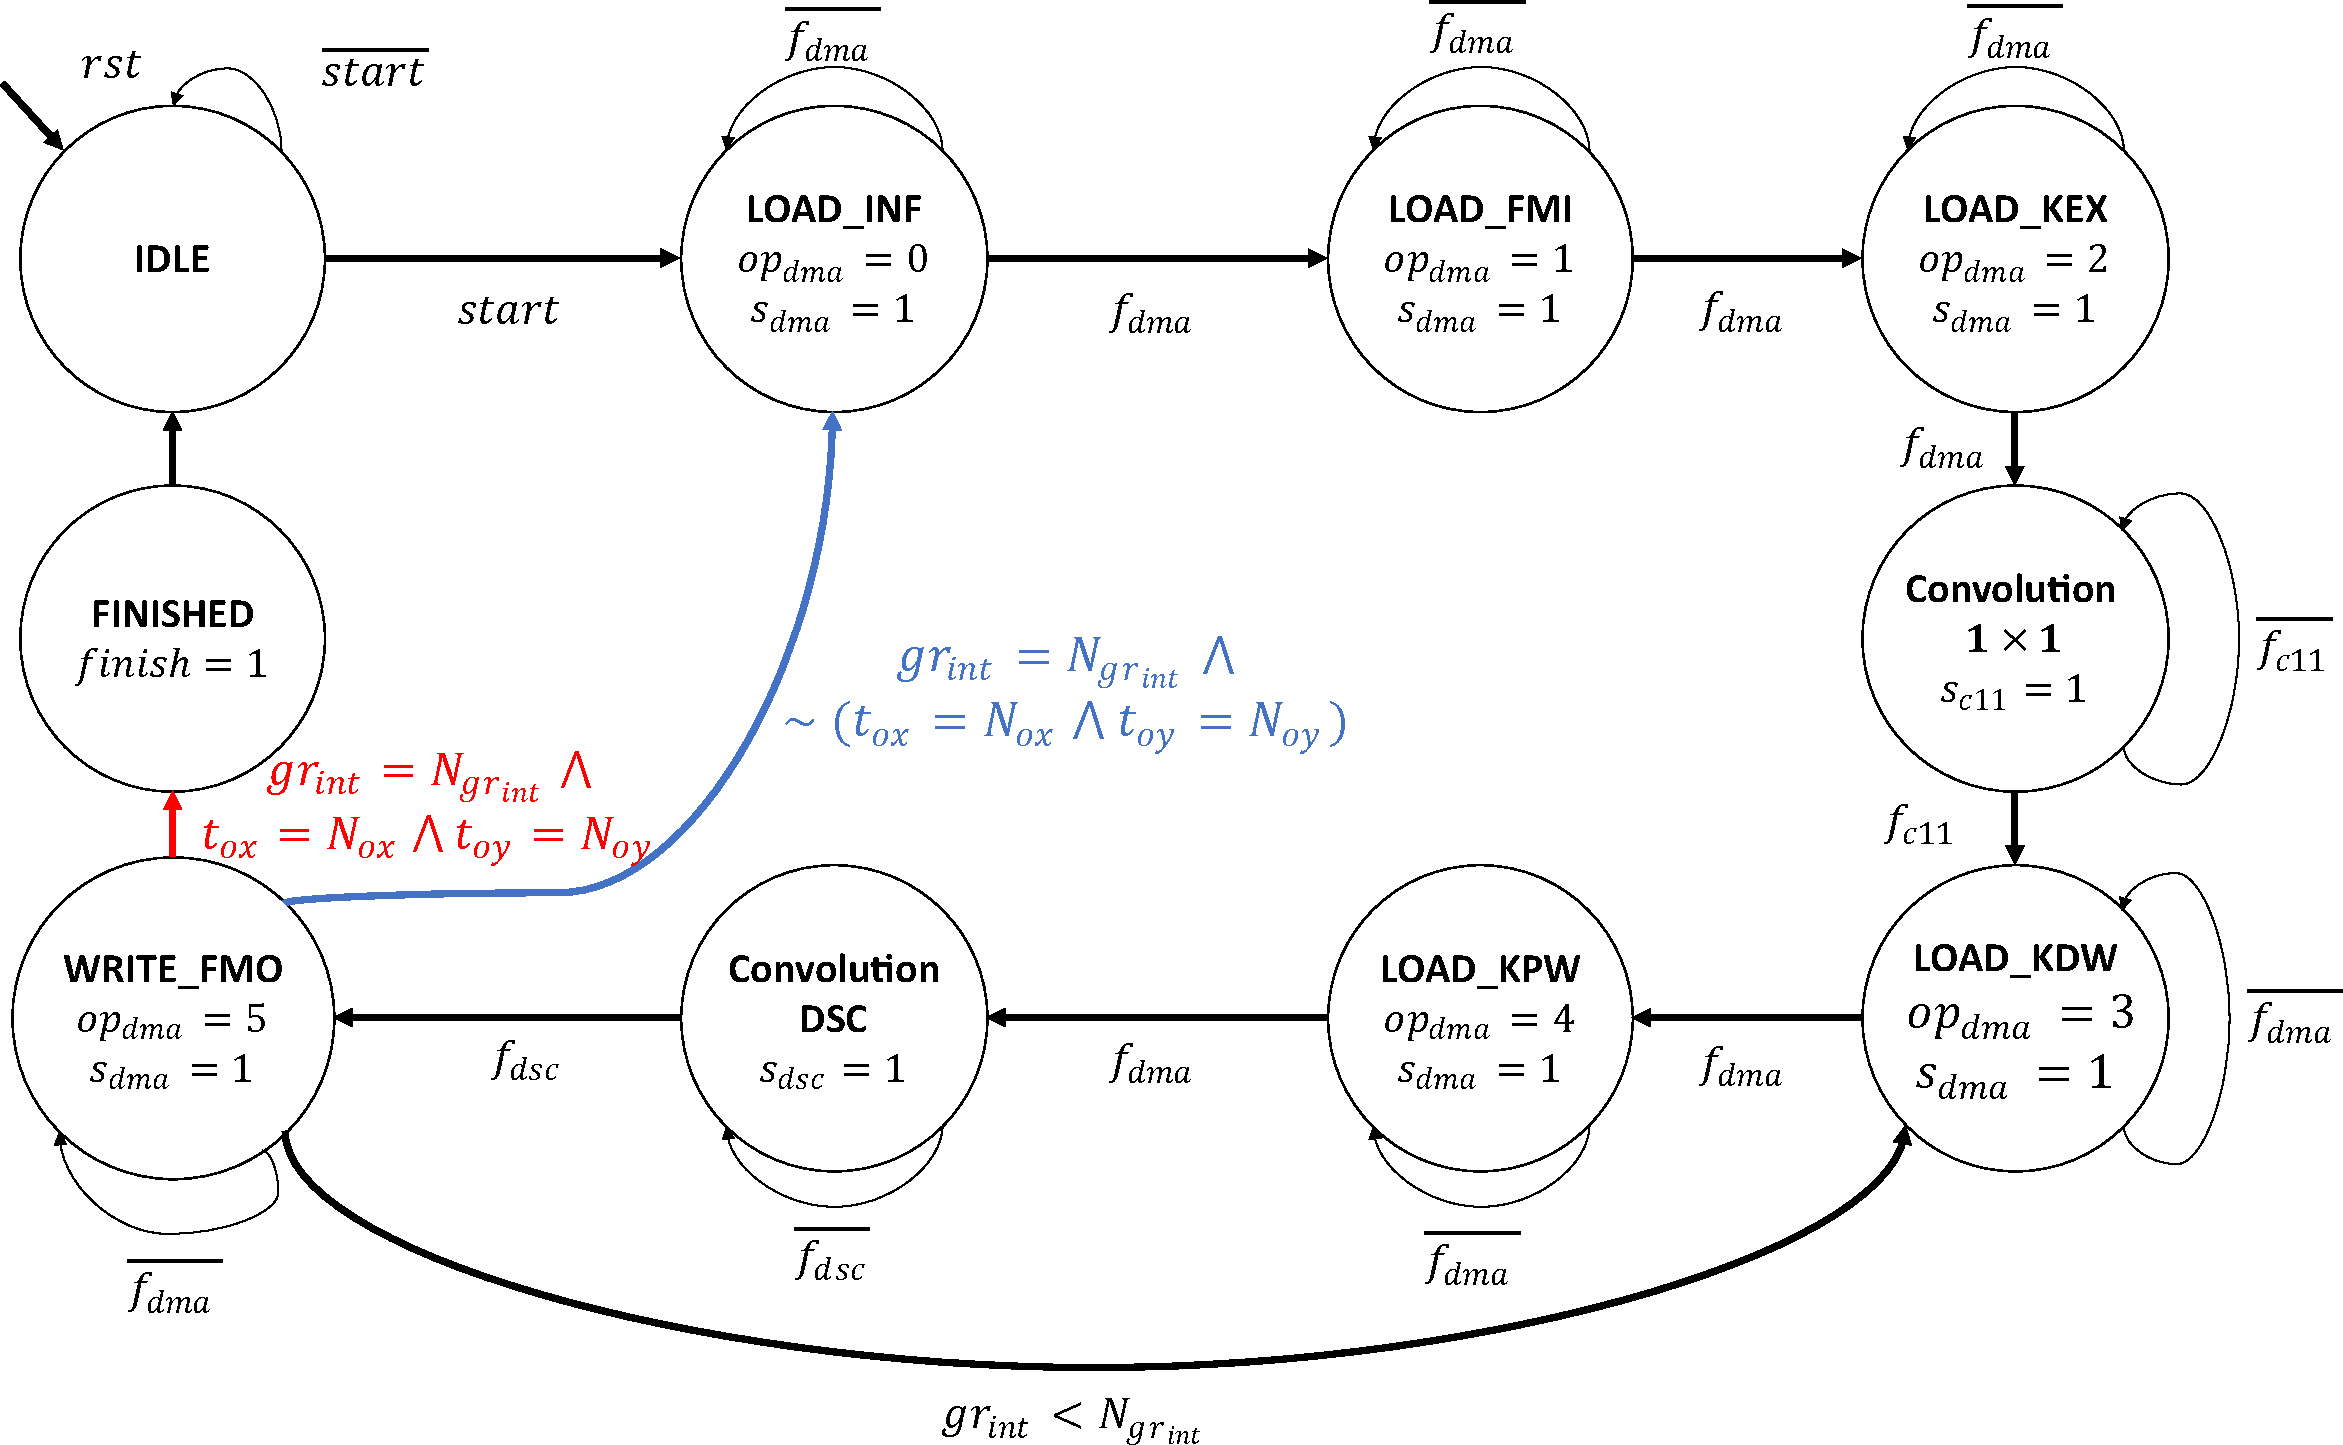
\includegraphics[width=\textwidth]{fsm-mc.pdf}
    \caption{\acrshort{fsm} of the main controller}
    \label{fig:fsm_mc}
\end{figure}
We can describe the behavior of the main controller using a \acrfull{fsm}, as illustrated in Figure \ref{fig:fsm_mc}. For the sake of clarity, additional informations transmitted to the components are not shown in the Figure. The \textbf{IDLE} state is the state where the main controller is waiting to perform a bottleneck convolution. Once the main controller has received a starting signal, it performs the following operations:
%
\begin{figure}
    \centering
    %
    \begin{subfigure}[t]{.49\textwidth}
        \centering
        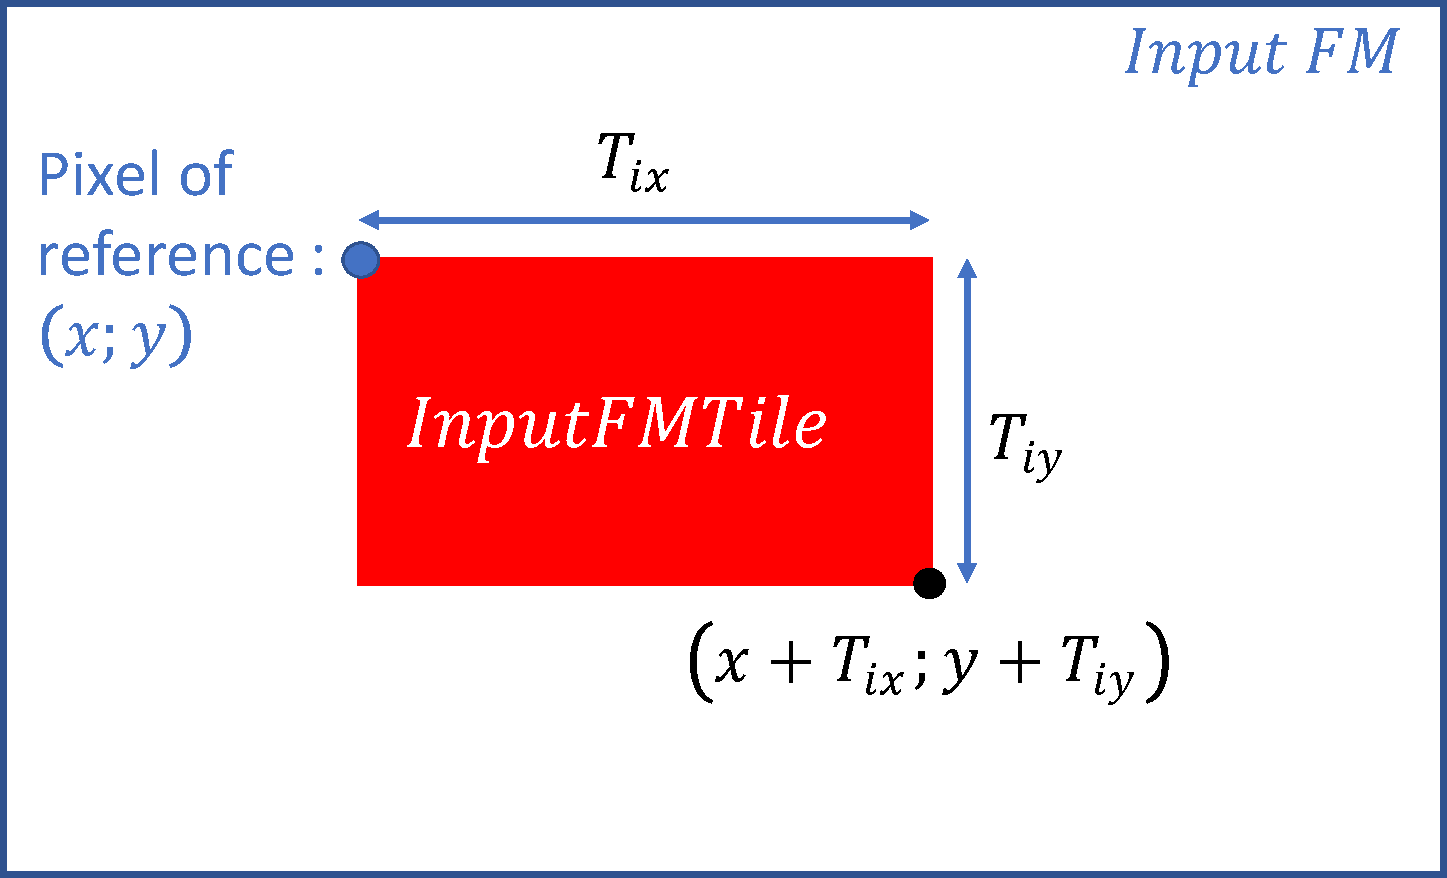
\includegraphics[width=\linewidth]{pixofref.pdf}
        \caption{Example of the pixel of reference for an input \acrshort{fm} tile}
        \label{fig:pix_of_ref}
    \end{subfigure}
    %
    \begin{subfigure}[t]{.49\textwidth}
        \centering
        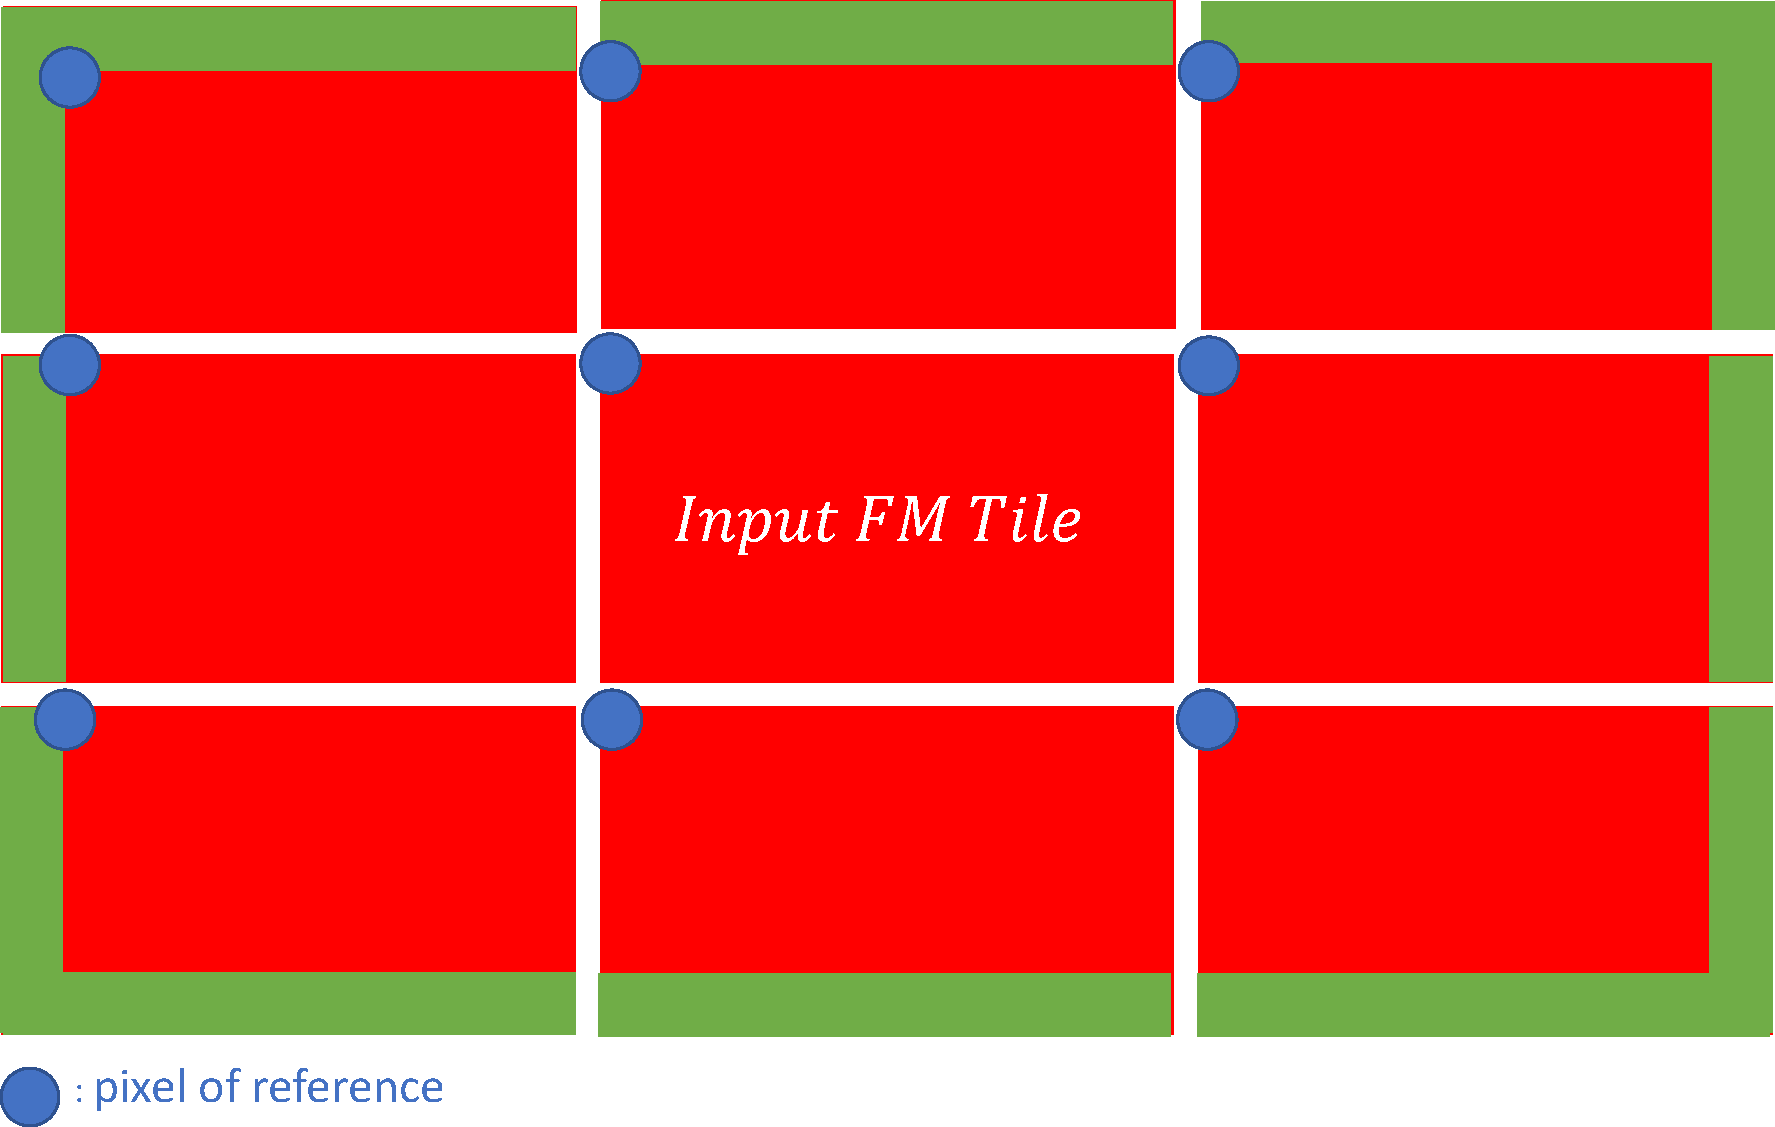
\includegraphics[width=\linewidth]{tilepadding.pdf}
        \caption{Padding configuration of input \acrshort{fm} tiles, where red area represent pixels fetched from external memory and green area represent padding pixels}
        \label{fig:tile_padding}
    \end{subfigure}
    %
    \caption{Illustration of the concept of the pixel of reference and padding}
\end{figure}
%
\begin{enumerate}
    \item \textbf{LOAD\_INF}: to perform the bottleneck convolution, the main controller first needs to fetch the layer information stored in the external memory. Therefore it tells the \acrshort{dma} to fetch them ($op_{dma} = 0$).
    %
    \item \textbf{LOAD\_FMI}: the bottleneck convolution starts by fetching a tile of inputs and weights from the main memory. As all inputs in the channel-axis are buffered (corresponding to all the fetching groups), an input \acrshort{fm} tile can be determined only by the spatial coordinates of the tile first element - pixel of reference (with the smallest $(x, y)$). Indeed, the \acrshort{dma} can fetch, for each channel, all pixels in the range $[(x, y); (x+T_{ix}, y+T_{iy})]$, which corresponds to the tile, as illustrated in Figure \ref{fig:pix_of_ref}.
    As a result, when the main controller asks the \acrshort{dma} to load into the on-chip memory a tile of input \acrshort{fm} ($op_{dma} = 1$), it also transfers the spatial coordinates and the memory address of its pixel of reference. Moreover, since we have to add padding to the tile (spatial dimensions are not reduced by the convolution operations), 0 value pixels are stored in the on-chip memory at corresponding positions when the reference pixel is on one edge of the input \acrshort{fm}, as shown in Figure \ref{fig:tile_padding}.
    %
    \item \textbf{LOAD\_KEX}: after fetching the input \acrshort{fm} tile, the main controller asks the \acrshort{dma} to load the $N_{par}$ $1 \times 1$ kernels into the on-chip memory ($op_{dma} = 2$), corresponding to the intermediate fetching group $group_{int}$. %Rajouter le channel de ref
    \item \textbf{CONV\_11}: after loading the weights and pixels, the $1 \times 1$ convolution can be performed. Once the $N_{par}$ intermediate channels corresponding to the intermediate fetching group $group_{int}$ have been produced, the \acrshort{dsc} can be executed.
    \item \textbf{LOAD\_KDW} and \textbf{LOAD\_KPW}: before doing the \acrshort{dsc}, the pointwise and depthwise kernels corresponding to the intermediate fetching group should be loaded by the \acrshort{dma} ($op_{dma} = 3$ and $op_{dma} = 4$).
    \item \textbf{CONV\_DSC}: all output \acrshort{fm} tile partial products can be computed by performing the \acrshort{dsc} on the $N_{par}$ intermediate channels. If all intermediate fetching groups have been processed, final results are computed and can be written into the external memory. Otherwise, the next $N_{par}$ intermediate channels should be computed. Moreover, since output \acrshort{fm} partial results will be kept in on-chip memory, the main controller indicates to the \acrshort{dsc} \acrshort{pe}s whether the values read from the \textit{FMO Buffer} should be consired as valid. If it is not the case, the value should be set to 0.
    \item \textbf{WRITE\_FMO}: this state indicates that there are only final results in the \textit{FMO Buffer}. The main controller tells the \acrshort{dma} that its content can be written to the external memory ($op_{dma} = 5$). As for the input \acrshort{fm} tiles, the output \acrshort{fm} tiles are determined by their pixel of reference, which is also transmitted to the \acrshort{dma}. If all tiles have been processed, the bottleneck convolution is completed and the main controller state turns to \textbf{FINISHED}. Otherwise, a new tile has to be processed and main controller returns to \textbf{LOAD\_FMI} state.
    \item \textbf{FINISHED}: The bottleneck convolution is done and the main controller sets the finish signal.
\end{enumerate}
%
\subsection{DMA}
%
The purpose of the \acrshort{dma} is to fill the \textbf{data buffer} with its corresponding tile fetched from external memory and write the output pixels into the external memory. Therefore, it has to manage six types of operation, referenced by its operation number $op_{dma}$:
%
\begin{itemize}
    \item $op_{dma} = 0$: Load the layer information
    \item $op_{dma} = 1$: Load an input \acrshort{fm} tile, referenced by its pixel of reference. The \acrshort{dma} needs as extra information the coordinate and the memory address of that pixel of reference.
    \item $op_{dma} = 2$: Load the $1 \times 1$ kernels used to produce the intermediate fetching group $group_{int}$ of size $N_{par}$. The \acrshort{dma} needs as extra information the first kernel and the memory address of its first weight to correctly load the $N_{par}$ kernels.
    \item $op_{dma} = 3$: Load the depthwise kernels corresponding to the intermediate fetching group $group_{int}$ of size $N_{par}$. The \acrshort{dma} needs as extra information the first kernel of the group and the memory address of its first weight to correctly load the $N_{par}$ kernels.
    \item $op_{dma} = 4$: Load the weight fetching group (of size $N_{np}$) of all pointwise kernels corresponding to the intermediate fetching group $group_{int}$. The \acrshort{dma} needs as extra information the position of the first weight in the fetching group and its memory address.
    \item $op_{dma} = 5$: Write the content of the \textbf{FMO Buffer} into the external memory, which corresponds to a tile of output \acrshort{fm}. As this tile is referenced by its pixel of reference, the \acrshort{dma} needs as extra information the coordinate and the memory address of that pixel of reference.
\end{itemize}

%
\begin{figure}
    \centering
    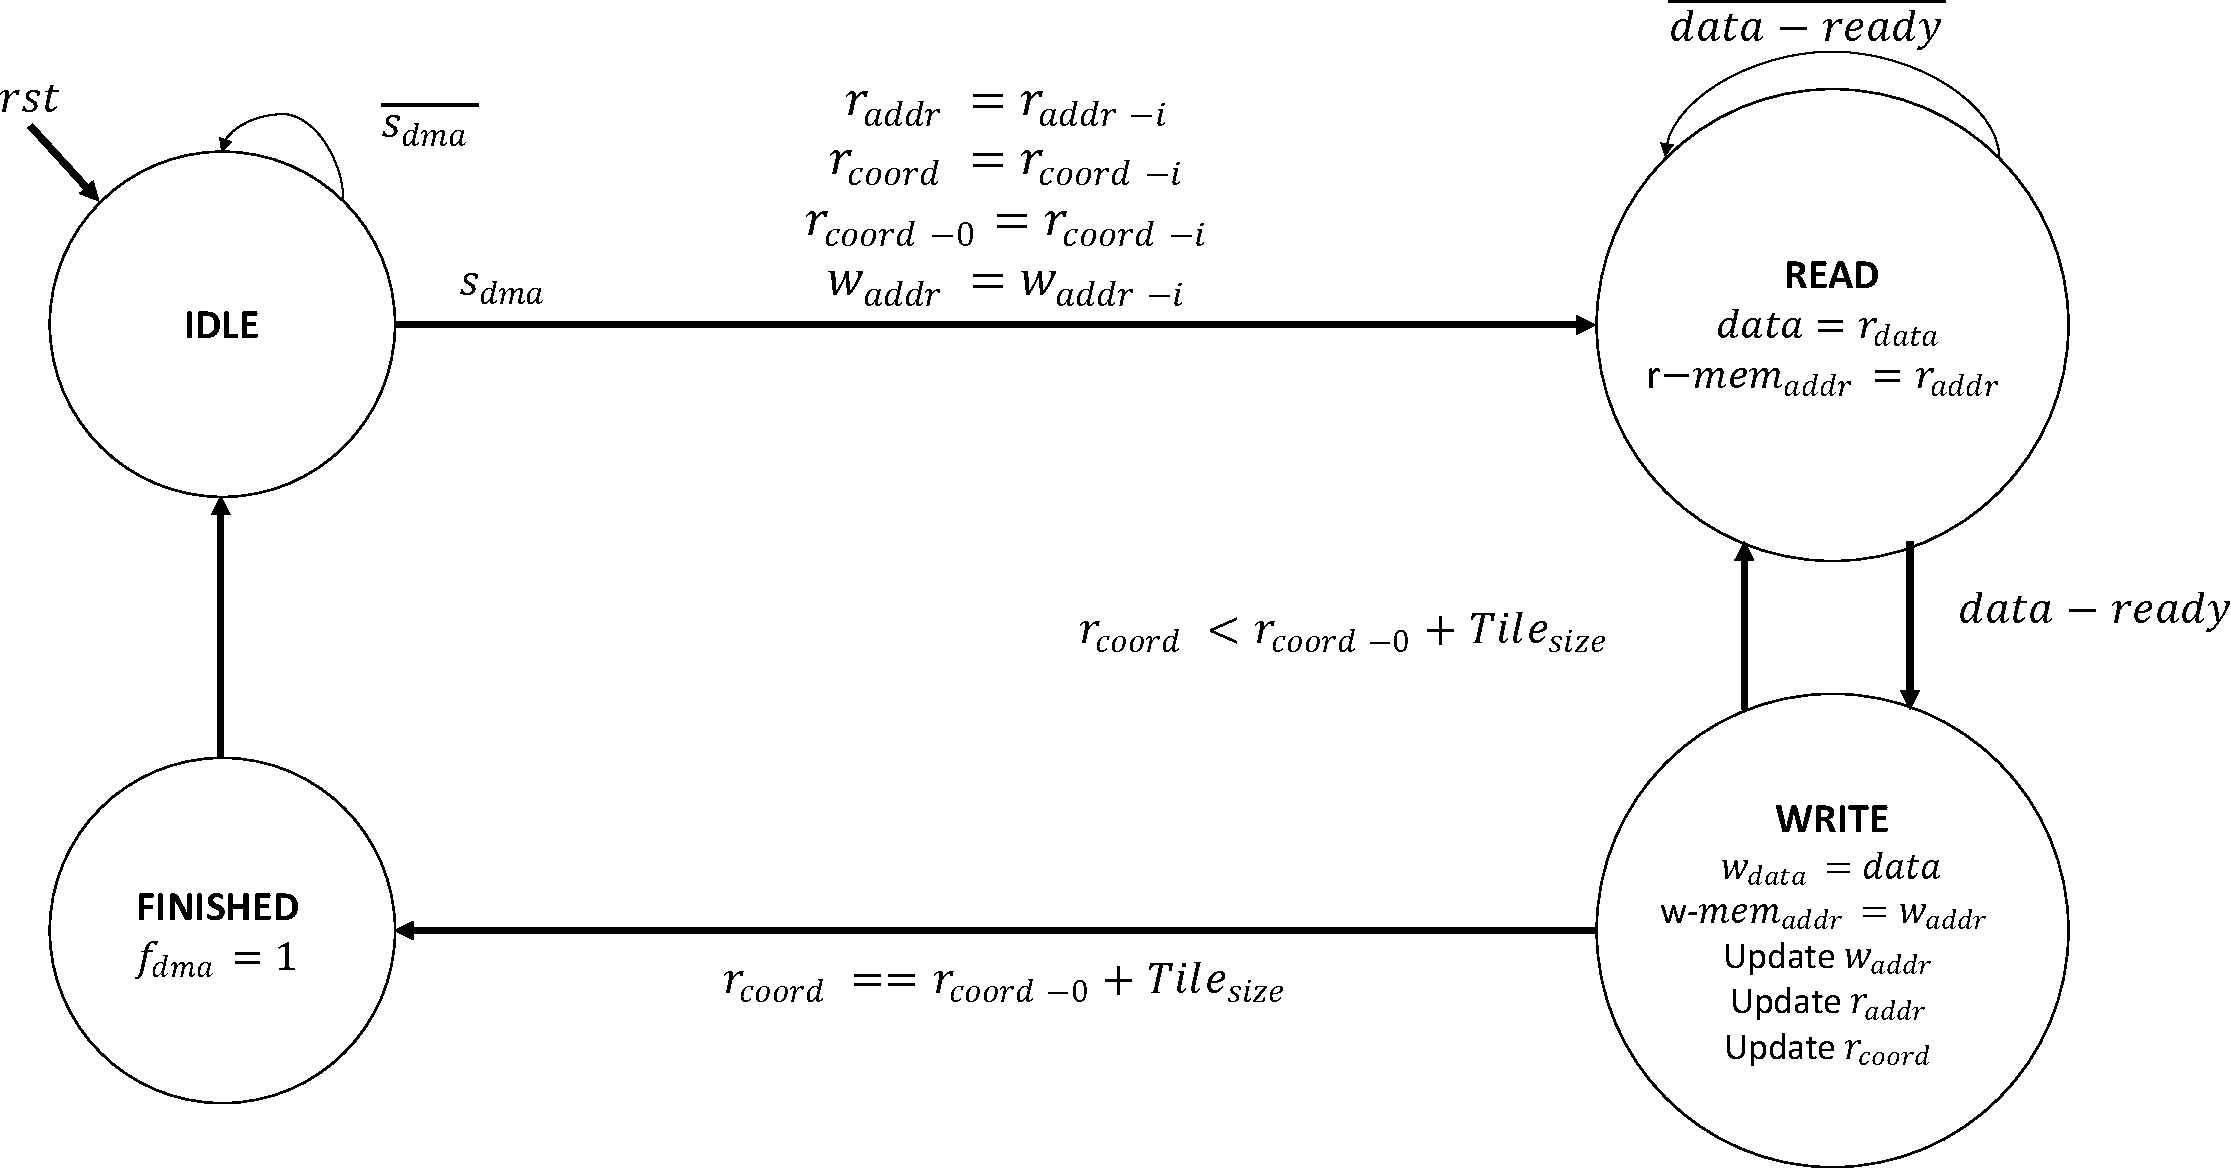
\includegraphics[width=\textwidth]{fsm-dma.pdf}
    \caption{\acrshort{fsm} of the \acrshort{dma}}
    \label{fig:fsm_dma}
\end{figure}
When the main controller asks the \acrshort{dma} for a transfer, it sets its start signal, which operation to execute ($op_{dma}$), and all extra information related to the external memory required. If the \acrshort{dma} reads or writes into a buffer, the initial address $r_{addr-i}/w_{addr-i}$ can be set to 0. Indeed, buffer addresses start from 0 to $Buffer_{N_{elem}} - 1$. The behavior of the \acrshort{dma} can be expressed using a \acrshort{fsm}, as found in Figure \ref{fig:fsm_dma}. A general \acrshort{fsm} has been illustrated because each operation shares the same structure. As the \acrshort{dma} only fetches data from one memory and writes the data into another one, each operation is composed of 2 states:
\begin{itemize}
    \item \textbf{READ}: the \acrshort{dma} fetches the required data at a address $r_{addr}$. Once the data is loaded by the \acrshort{dma}, it moves to the next state to write the data in the on-chip memory. When loading the input \acrshort{fm} tile, if the address corresponds to a padding pixel, the value to write is 0 and the \acrshort{dma} directly moves to the \textbf{WRITE} state. If the data is fetched from the external memory, the \acrshort{dma} sets the read request signal $r_{request_{extmem}}$ (enabling a transfet) waits the data read from the external memory to be valid ($r_{valid_{extmem}}$). But if the data is fetched from a buffer, the process can be pipelined. That is why, before the \acrshort{dma} reads data from the on-chip memory, it is in a state called \textbf{RAM\_LOADING} to initialize the pipeline process.
    \item \textbf{WRITE}: the \acrshort{dma} sends a write signal and the associated data $w_data$ and address $w_{address}$ to the corresponding memory . If the operation is finished (the tile has been fetches), the \acrshort{dma} goes into the \textbf{FINISHED} state. Otherwise, it updates the address of the next data to fetch and goes back to the \textbf{READ} state.
\end{itemize}

The \acrshort{dma} has therefore signals for reading $r_{extmem}$ a data at address $address_{extmem}$. Since the \acrshort{dma} performs one transfer at a time, we can share the fetched data (to be written) $w_{data}$ between all memory component and we set the write signal to the corresponding component. In a similar way, the signal to access or write data in a buffer $ram_{addr}$ can also be shared between the different buffers. As the \acrshort{dma} reads the contrent of only one buffer, we define the corresponding signal as $r_{ram}$ (and hence at address $ram_{addr}$).
%
\subsection{1\texttimes1 convolution PE}
%
\begin{figure}
    \centering
    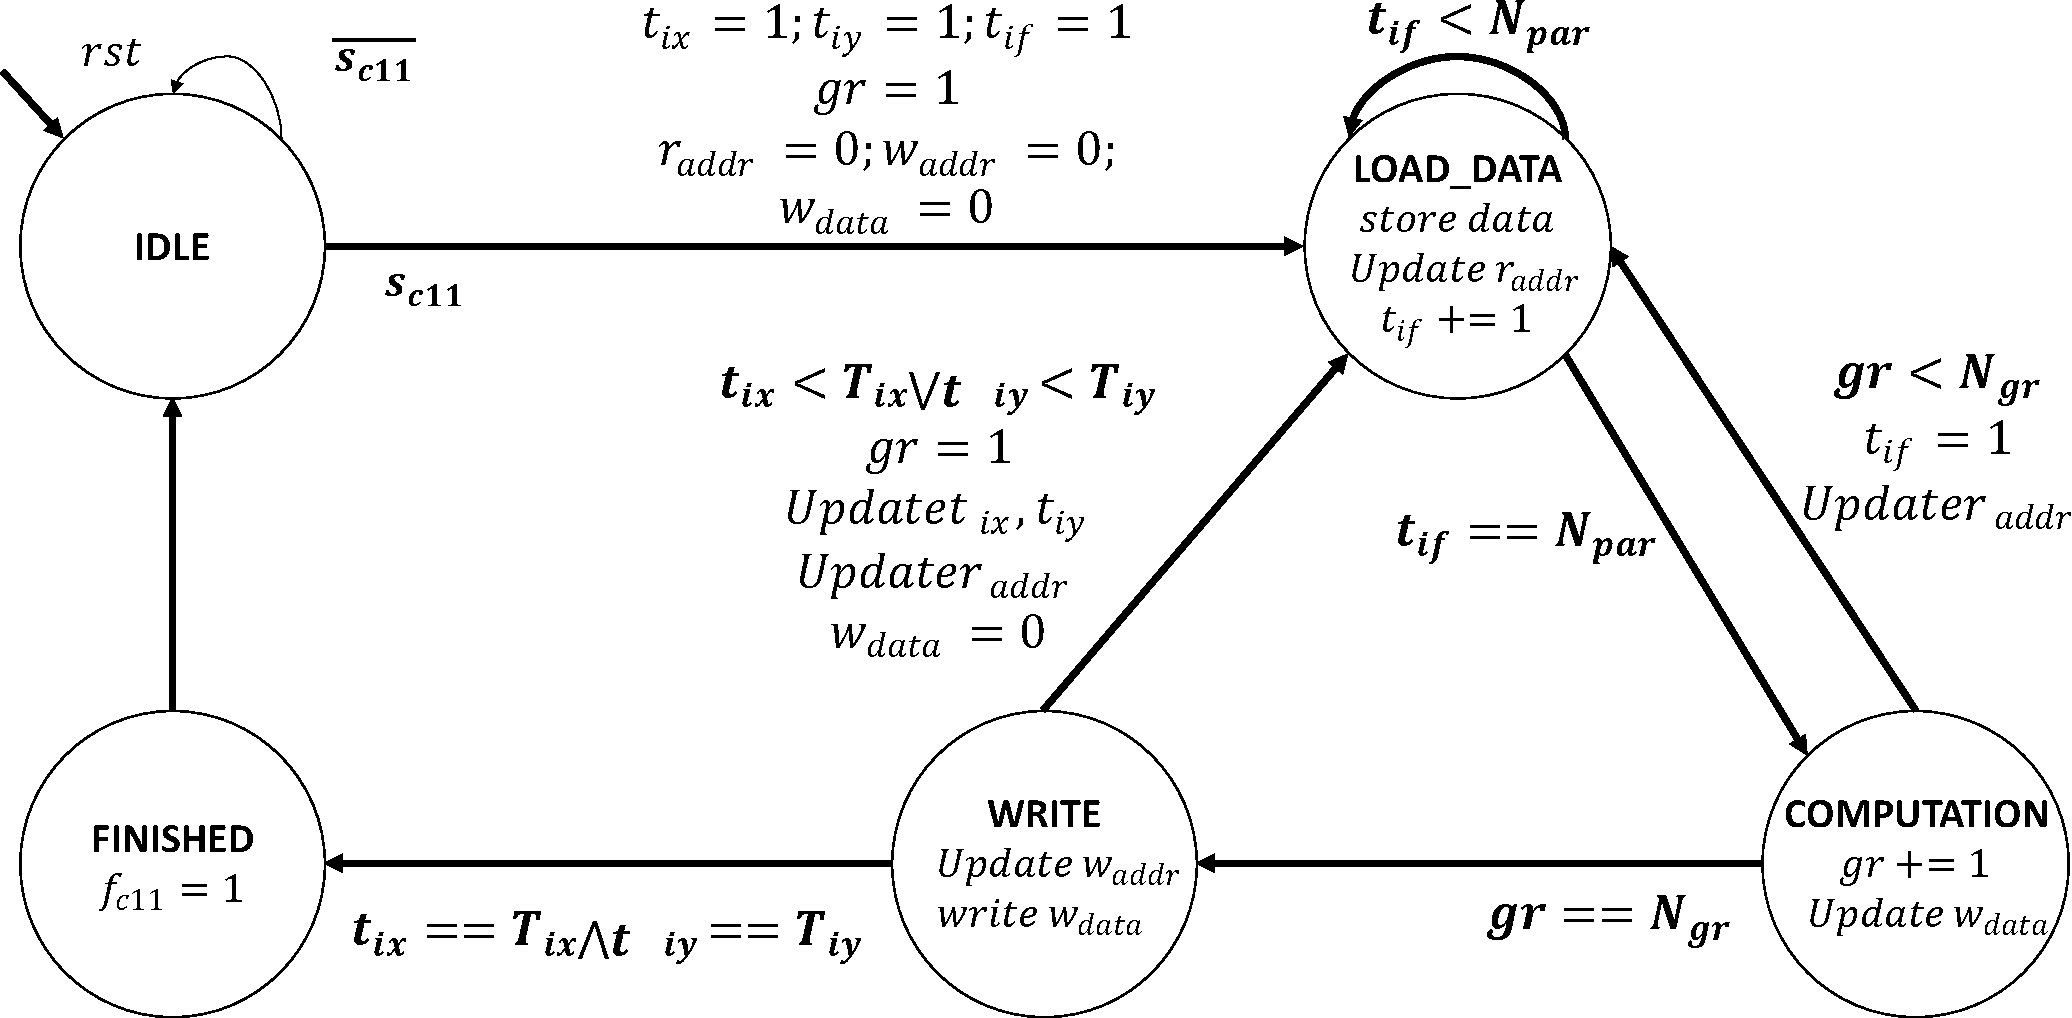
\includegraphics[width=\textwidth]{fsm-c11.pdf}
    \caption{\acrshort{fsm} of the 1\texttimes1 convolution PE}
    \label{fig:fsm_c11}
\end{figure}
%
The purpose of this component is to execute the Algorithm \ref{pseudocode:c11}. The behavior of the \acrshort{pe} can be expressed using a \acrshort{fsm}, as found in Figure \ref{fig:fsm_c11}.

\begin{figure}
    \centering
    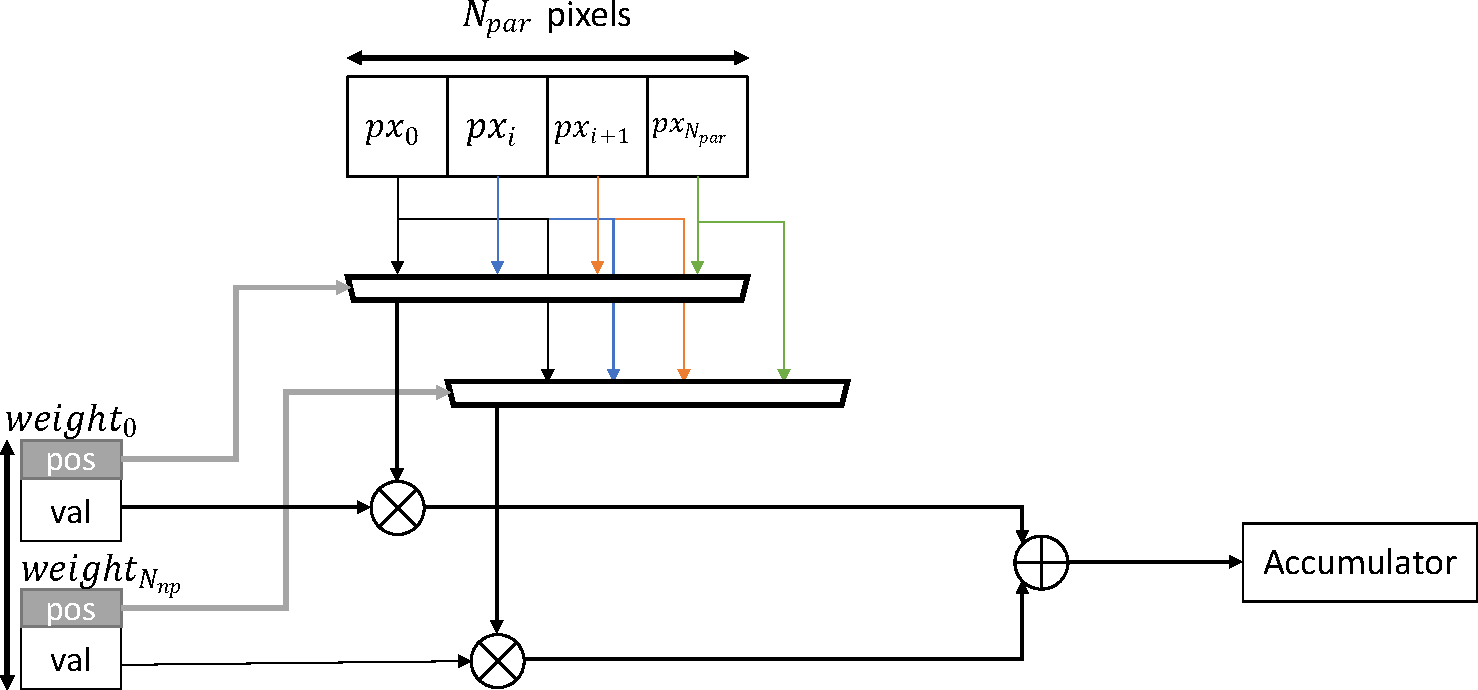
\includegraphics[width=\linewidth]{hardware_conv11.pdf}
    \caption{\acrshort{pe} structure performing the convolution where $N_{par} = 4$ and $N_{np} = 2$, inspired by \cite{kang_accelerator-aware_2020}}
    \label{fig:c11_hardware}
\end{figure}
%
When the \acrshort{pe} receives a starting signal, it means that the \textbf{FMI} and \textbf{KEX BUFFERS} contain the data to execute the next $1 \times 1$ convolution. For each fetching group corresponding to an intermediate pixel at address $w_{addr}$, the \acrshort{pe} loads the corresponding $N_{par}$ inputs and $N_{np}$ weights into its registers (\textbf{LOAD\_DATA} state).
Once it is done, the computation can be performed (\textbf{COMPUTATION} state). Since the convolution is fully-unrolled, we can use the \acrshort{pe} structure from \textcite{kang_accelerator-aware_2020}, which is shown in Figure \ref{fig:c11_hardware}. The output result is then summed with the content of the accumulator (which contains 0 for the first fetching group).

When the convolution is done for one intermediate pixel, the result is fed to the ReLU6 activation (see Section \ref{subs:acti}), and its output is written into the \textbf{FMINT BUFFER}. If all pixels required for the \acrshort{dsc} have been computed, the \acrshort{pe} sends an ending signal to the main controller (\textbf{FINISHED} state). Otherwise it computes the next intermediate pixel.

This \acrshort{pe} is described for the its use in the bottleneck convolution, but is could also be used in the $1 \times 1$ layers.
%
\subsection{DSC PE}
%
\begin{figure}
    \centering
    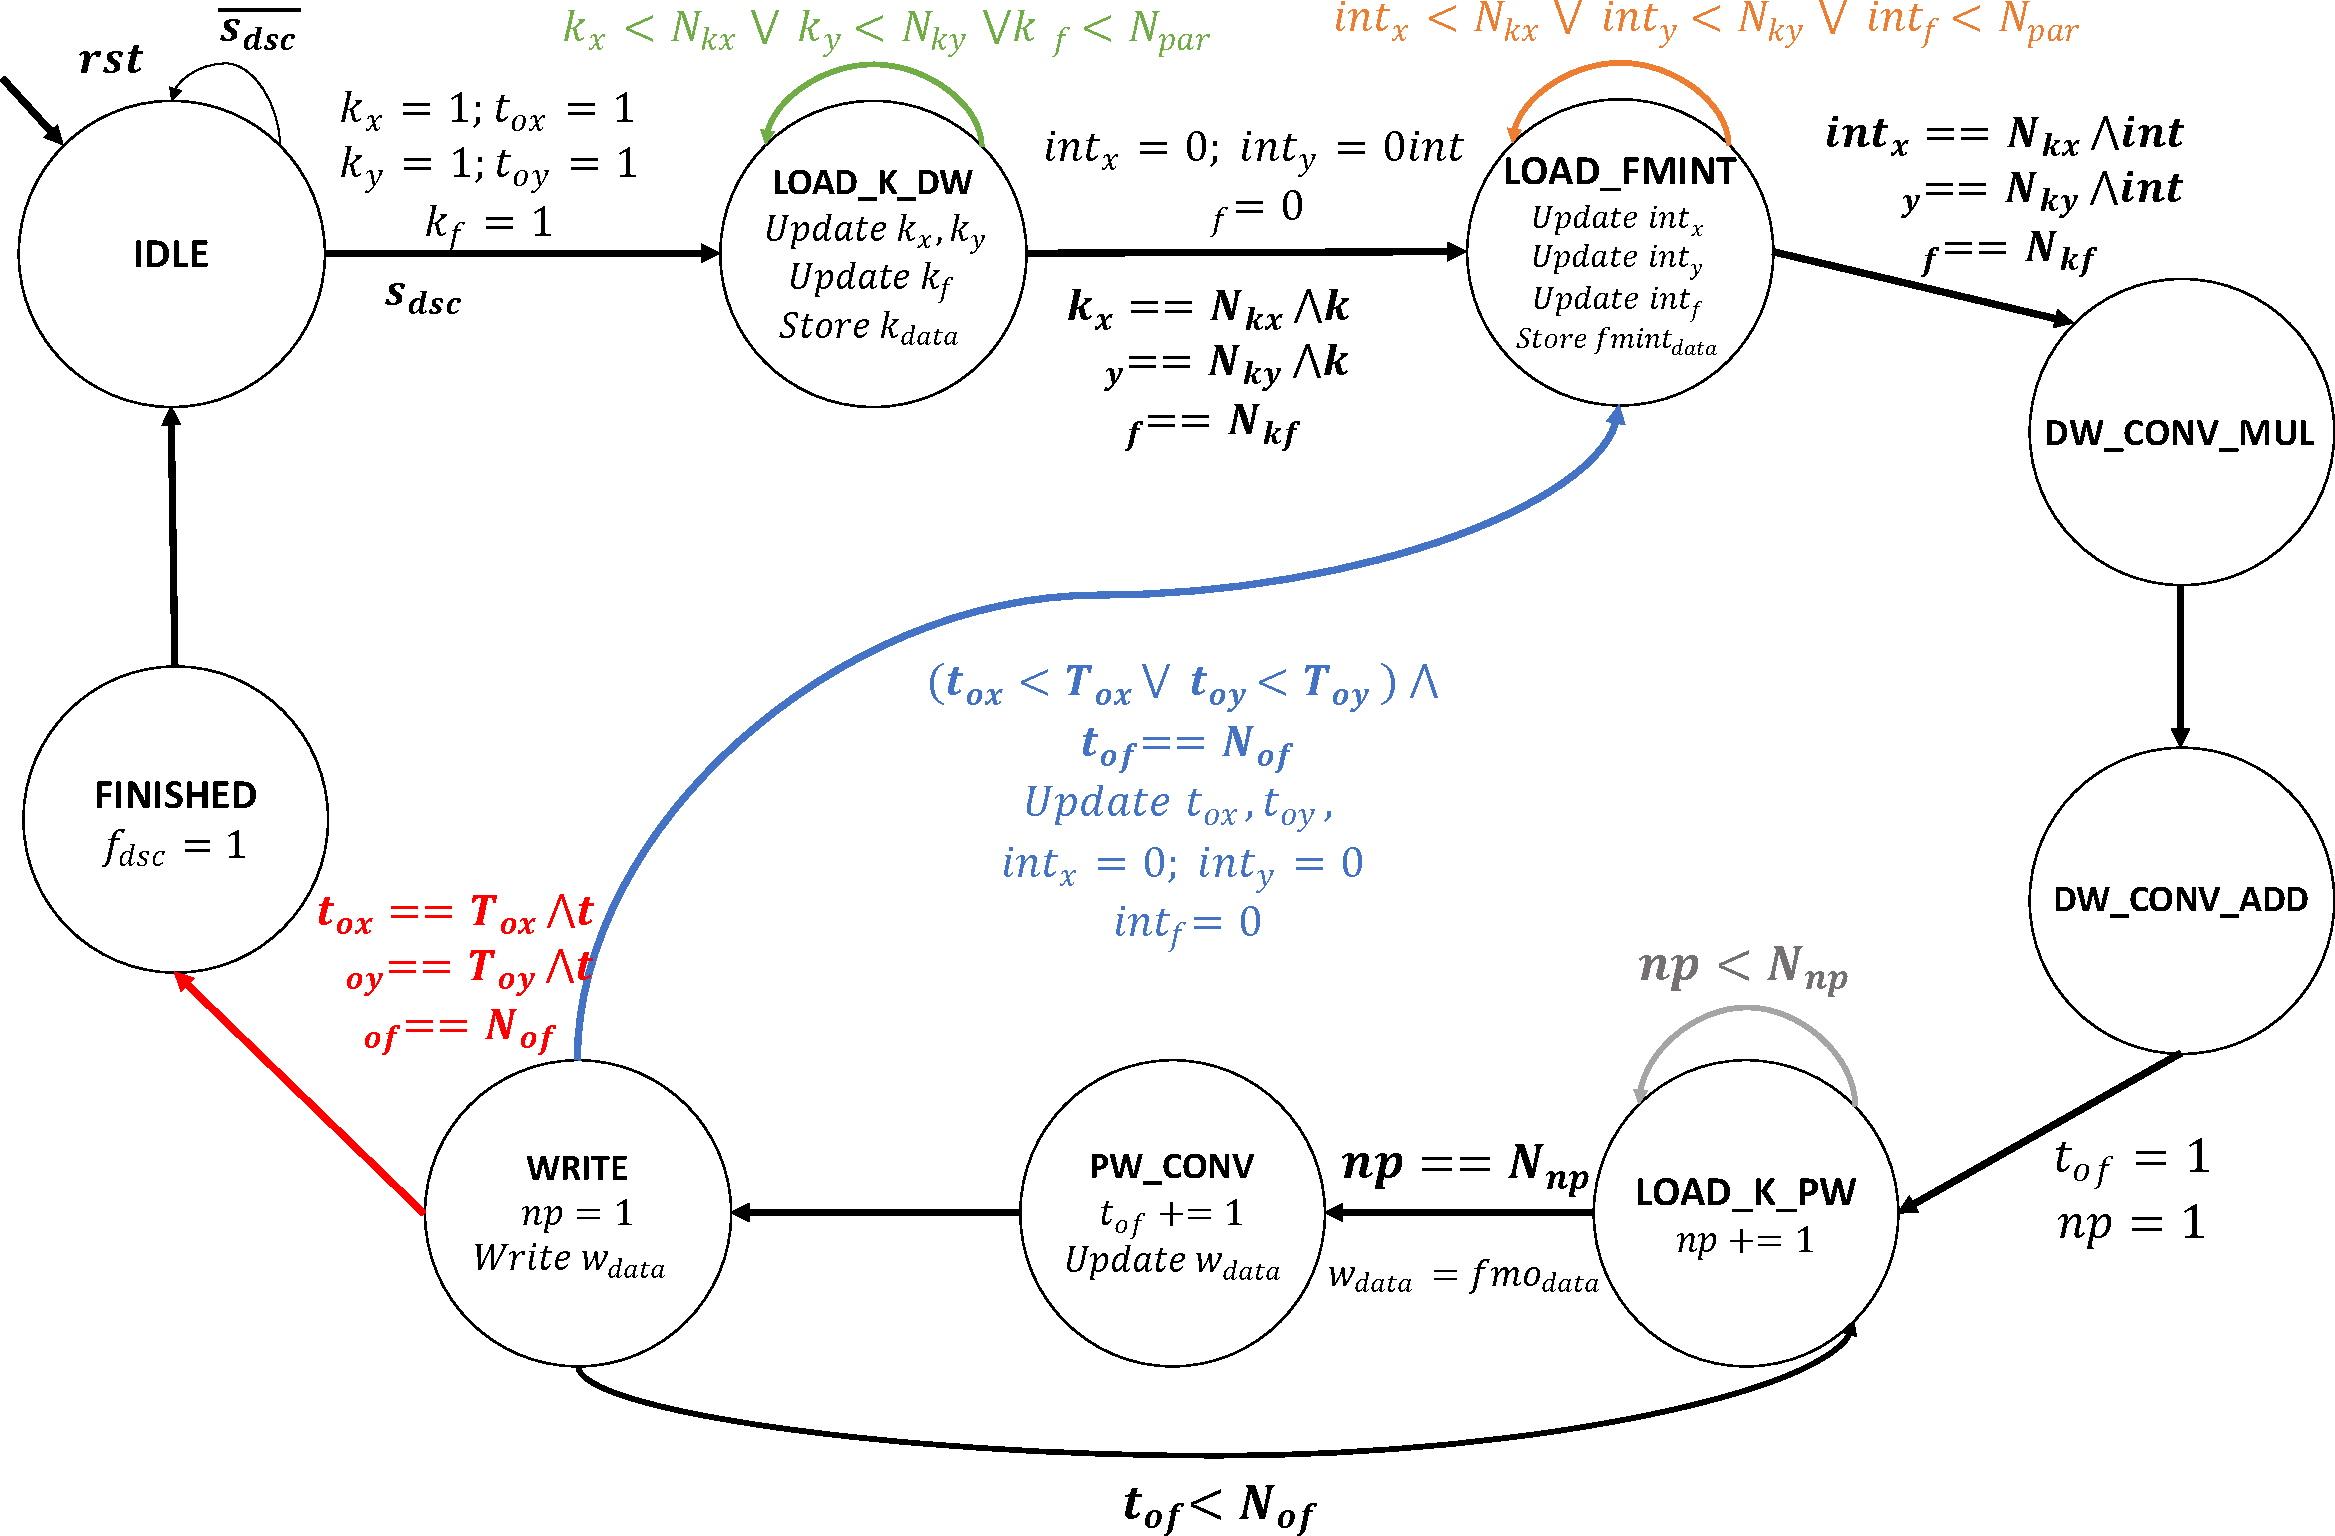
\includegraphics[width=\textwidth]{fsm-dsc.pdf}
    \caption{\acrshort{fsm} of the \acrshort{dsc} \acrshort{pe}}
    \label{fig:fsm_dsc}
\end{figure}
This \acrshort{pe} is designed to perform the \acrshort{dsc}. Once the $1 \times 1$ convolution has computed the next intermediate fetching group and the \textbf{Buffers} containts the required data, we can do the \acrshort{dsc} as in Algorithm \ref{pseudocode:dsc}. The \acrshort{pe} can be described as a \acrshort{fsm} executing the proposed algorithm in Figure \ref{fig:fsm_dsc}.

\begin{figure}
    \centering
    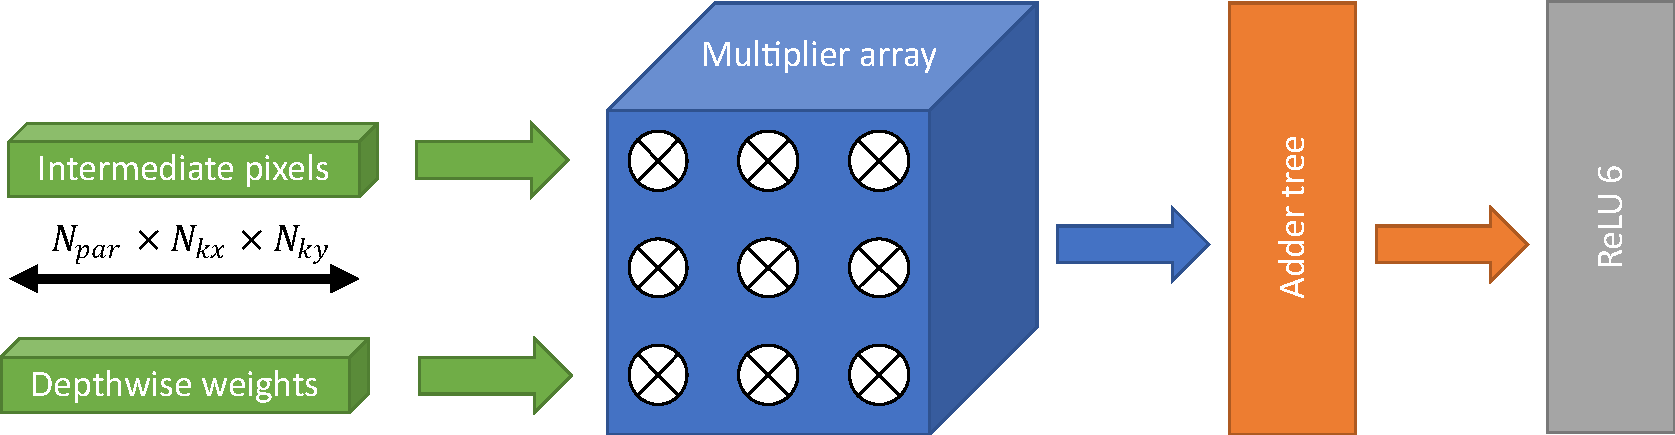
\includegraphics[width=\textwidth]{hardware-dw.pdf}
    \caption{\acrshort{pe} structure performing the depthwise convolution, inspired by \cite{bai_cnn_2018}}
    \label{fig:dsc_hardware}
\end{figure}
%
The \acrshort{pe} has the same structure as the 1\texttimes1 convolution PE. However, the 2 \acrshort{pe}s diverges on the following elements:
\begin{itemize}
    \item For each intermediate pixels, the 1\texttimes1 \acrshort{pe} performs $N_{gr}$ $1 \times 1$ partial convolutions on the input pixels and $1 \times 1$ kernels directly fetched from the buffers.
    %
    \item On the other hand, for the \acrshort{dsc} \acrshort{pe} must first loads the $N_{kx} \times N_{ky} \times N_{par}$ intermediate pixels and depthwise weights (\textbf{LOAD\_K\_DW} and \textbf{LOAD\_FMINT} states). This is done in two different states because the depthwise is fully-unrolled and therefore we keep all required weights into the registers. We have to only fetch them once from the external memory.
    %
    \item After it has loaded the input pixels and the depthwise weights, the depthwise convolution can be performed. To execute the depthwise convolution for each intermediate channels, we can use the same \acrshort{pe} as \textcite{bai_cnn_2018}, as illustrated in Figure \ref{fig:dsc_hardware}. First we do a element-wise multiplication using a multiplier array between pixels and weights (\textbf{DW\_CONV\_MUL} state). Then, we simply have to sum the products belonging to the same channel to obtain the $N_{par}$ depthwise produtcs used as input for the pointwise convolution (\textbf{DW\_CONV\_ADD} state). Then the registers store the results of the ReLU6 activation function for the \acrshort{dsc}.
    %
    \item We can perform the partial \acrshort{dsc} for the $N_{of}$ channels of spatial coordinate $o_x, o_y$. For each channel, we load the $N_{np}$ weights corresponding to that channel and the intermediate fetching group (\textbf{LOAD\_K\_PW} state). We also load the partial sum stored in the \textbf{FMO Buffer} to sum it with the results of the convolution (\textbf{PW\_CONV} state). However, if it is the first intermediate fetching group, this value is set to 0 ($first\_par\_i$ signal, set by the main controller).
    The structure of the \acrshort{pe} performing the pointwise convolution is the same as Figure \ref{fig:c11_hardware}. Then the sum between the partial sum stored and the result of the convolution is stored in the \textbf{FMO Buffer} (\textbf{WRITE} state).
    %
    \item When all the partial sum have been produced, the \acrshort{pe} moves to the \textbf{FINISHED} state and sets its finishing signal.
\end{itemize}

The \acrshort{dsc} \acrshort{pe} could be extended to support the standard, as pointed out by \textcite{bai_cnn_2018}. Indeed, if we consider sum all products in the multiplier array instead of only those belonging to the same channel, we perform the standard convolution.
%
\subsection{Buffer}
%
\begin{figure}
    \centering
    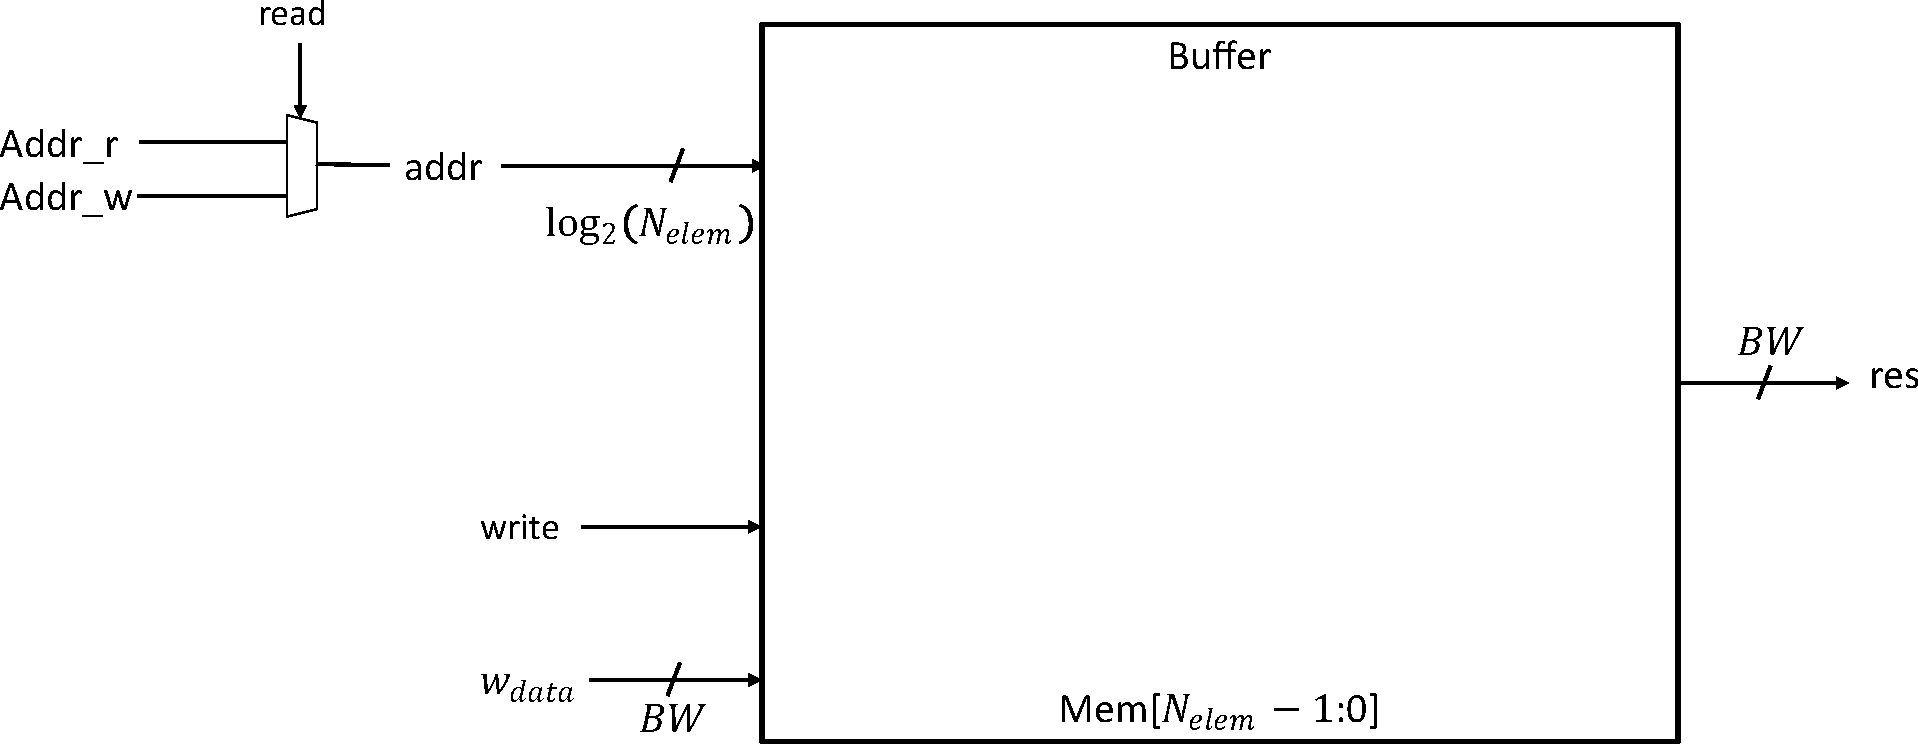
\includegraphics[width=\textwidth]{struct_ram.pdf}
    \caption{General architecture of a buffer component}
    \label{fig:struct_ram}
\end{figure}
%
The buffers compose the on-chip memory of the \acrshort{fpga}. As mentionned previously, the structure is composed of six buffers that share the same structure, as illustrated in Figure \ref{fig:struct_ram}. At each clock period, the output signal $res$ is equal to the value stored at address $addr$, or if the write signal $write$ is enabled, the value that is currently written. In the same way, if the write signal is set, the value in the buffer at address $addr$ is equal to the input data $w_{data}$. As multiple components may read or write a same buffer, a multiplexer is added to select from which address to read.

The value of $addr_r$ and $addr_w$ depend on the type of buffer. For \textbf{data buffer} the $addr_r$ is the \acrshort{pe} address of the corresponding buffer, and $addr_w$ is the \acrshort{dma} $ram_{addr}$ signals. For \textbf{result buffer}, $addr_w$ is the corresponding \acrshort{pe} output address and $addr_r$ can be either a \acrshort{pe} address requesting a result (\textbf{FMINT Buffer}) or the \acrshort{dma} $ram_{addr}$ signals to write final results to external memory ((\textbf{FMO Buffer}))

However, the differences between each buffer are the maximum number of elements that can be stored $N_{elem}$ and the bitwidth $BW$ of their data stored. We explore for each buffer these two parameters.
\begin{itemize}
    \item \textbf{FMI Buffer}: we have determined from the loops analysis that we buffer each input \acrshort{fm} fetching group. Since the number of input \acrshort{fm} channels vary accross the different layers of the network, we can determine $N_{elem}$ using Equation \eqref{eq:nelem-fmi}. The number of bits to store a pixel is equal to $BW_{pixel}$. We can therefore express $BW$ such as Equation \eqref{eq:bw-fmi}.
    \begin{equation}
        N_{elem-fmi} = \forall l \in layers: Max\left( N_{if}^l \times Min\left(T_{ix}, N_{ix}^l\right) \times Min\left(T_{iy}, N_{iy}^l\right) \right)
        \label{eq:nelem-fmi}
    \end{equation}
    \begin{equation}
        BW_{fmi} = BW_{pixel}
        \label{eq:bw-fmi}
    \end{equation}
    %
    \item \textbf{KEX Buffer}: this buffer stores the $N_{par}$ $1 \times 1$ kernels required to perform this convolution, which expands the number of input channels. Therefore, we can express $N_{elem}$ using Equation \eqref{eq:nelem_kex}, where $N_{gr-max} = \left\lceil \frac{1280}{Npar} \right\rceil$ is the maximum number of fetching group in the whole network. Since the weights are expressed in the proposed compressed format, we also have to store the weight position in the fetching group.
    As a result, $BW$ can be expressed using Equation \eqref{eq:bw-kex}, where $BW_{weight}$ is the number of bits to represent a weight and $log_2(N_{par})$ the number of bits to represent the position.
    \begin{equation}
        N_{elem-kex} = N_{par} \times N_{np} \times N_{gr-max}
        \label{eq:nelem_kex}
    \end{equation}
    \begin{equation}
        BW_{kex} = BW_{weight} + log_2(N_{par})
        \label{eq:bw-kex}
    \end{equation}
    %
    \item \textbf{FMINT Buffer}: since the \acrshort{dsc} needs $N_{par}$ intermediate \acrshort{fm} channels and the $1 \times 1$ convolution does not reduce the spatial dimension of the input \acrshort{fm}, we can express the $N_{elem}$ using Equation \eqref{eq:nelem_fmint}. The bitwidth of a pixel is the bitwidth used to represent a pixel, as in Equation \eqref{eq:bw-fmint}.
    \begin{equation}
        N_{elem-fmint} = N_{par} \times T_{iy} \times T_{ix}
        \label{eq:nelem_fmint}
    \end{equation}
    \begin{equation}
        BW_{fmi} = BW_{pixel}
        \label{eq:bw-fmint}
    \end{equation}
    %
    \item \textbf{KDW Buffer}: applying the same methodoly as \textbf{FMINT Buffer} and since the depthwise kernels are fully buffered, we can express the $N_{elem}$ using Equation \eqref{eq:nelem_kdw}. The bitwidth of a pixel is the bitwidth used to represent a weight, as in Equation \eqref{eq:bw-kdw}.
    \begin{equation}
        N_{elem-kdw} = N_{par} \times N_{ky} \times N_{kx}
        \label{eq:nelem_kdw}
    \end{equation}
    \begin{equation}
        BW_{kdw} = BW_{weight}
        \label{eq:bw-kdw}
    \end{equation}
    %
    \item \textbf{KPW Buffer}: for each time we perform a \acrshort{dsc}, we need to convolve in each pointwise the corresponding weight fetching group with $N_{np}$ pixels in the $N_{par}$ channels. The maximum number of elements in the buffer can be computed using Equation \eqref{eq:nelem_kpw}. As the pointwise convolution is a $1 \times 1$ convolution, the bitwidth associated to each pointwise kernel is the same as the \textbf{KPW Buffer}, and can be expressed using Equation \ref{eq:bw-kpw}
    \begin{equation}
        N_{elem-kpw} = N_{np} \times N_{of}
        \label{eq:nelem_kpw}
    \end{equation}
    \begin{equation}
        BW_{kpw} = BW_{weight} + log_2(N_{par})
        \label{eq:bw-kpw}
    \end{equation}
    %
    \item \textbf{FMO Buffer}: using the same methodoly as for determining $N_{elem}$ and $BW$ for the \textbf{FMI Buffer}, they are expressed using Equation \eqref{eq:nelem_fmo} and \eqref{eq:bw_fmo}
    \begin{equation}
        N_{elem-fmo} = \forall l \in layers: Max\left( N_{of}^l \times Min\left(T_{oy}, N_{oy}^l\right) \times Min\left(T_{ox}, N_{ox}^l\right) \right)
        \label{eq:nelem_fmo}
    \end{equation}
    \begin{equation}
        BW_{fmo} = BW_{pixel}
        \label{eq:bw_fmo}
    \end{equation}
\end{itemize}

%
%
\section{Results and discussion} \label{sec:measure}
blabla

%
%
\afterpage{\blankpage}
\cleardoublepage
\newpage
